\documentclass{bmstu}

\usepackage{graphicx}
\usepackage{longtable}
\usepackage{listings}
\usepackage{xcolor}
\RequirePackage[listings]{tcolorbox}
\tcbuselibrary{listings,breakable,minted,skins}

\bibliography{biblio}
\setlist[itemize]{label=---}

\newtcbinputlisting[auto counter,number within=chapter]{\sourcelisting}[4][]{
	enhanced,
	before={\par\medskip\noindent Листинг~\thetcbcounter~--~#3\par\nobreak\vspace{2pt}},
	after={\par\medskip},
	arc=0mm,
	boxrule=1pt,
	listing only,
	listing file={#2},
	listing engine=minted,
	minted language=csharp,
	minted options={
		linenos,
		breaklines=true,
		breakanywhere=true,
		breakbefore=.,
		breakafter={,()[]},
		fontsize=\small\ttfamily,
		numbersep=1.5mm,
		firstnumber=1,
		escapeinside=~~,
		#1
	},
	colback=white,
	colframe=black,
	breakable,
	enlarge top at break by=5mm,
	overlay first={
		\draw[line width=.5pt] (frame.south west)--(frame.south east);
	},
	overlay middle={
		\draw[line width=.5pt] (frame.south west)--(frame.south east);
		\draw[line width=.5pt] (frame.north west)--(frame.north east);
		\node[anchor=south west, inner xsep=0pt, xshift=0pt] at (frame.north west) {Продолжение листинга \thetcbcounter};
	},
	overlay last={
		\draw[line width=.5pt] (frame.north west)--(frame.north east);
		\node[anchor=south west, inner xsep=0pt, xshift=0pt] at (frame.north west) {Окончание листинга \thetcbcounter};
	},
	label={#4}
}

\begin{document}

\makethesistitle
	{Информатика и системы управления}
	{Программное обеспечение ЭВМ и информационные технологии}
	{Метод обеспечения согласованности состояний двух асинхронных игроков с помощью конечных автоматов}
	{В.~А.~Лукьяненко/ИУ7-81Б}
	{Д.~А.~Кузнецов}
	{}{}

\setcounter{page}{5}
\begin{essay}{}
	Расчетно-пояснительная записка содержит \pageref{LastPage} страниц, 4 раздела, 7 рисунков, 10 таблиц, 19 использованных источников, 1 приложение.

	В работе представлена разработка метода обеспечения согласованности состояний двух асинхронных игроков с помощью конечных автоматов. Проведен анализ подходов к синхронизации игровых состояний и передаче данных в многопользовательских приложениях, рассмотрены причины рассинхронизации при UDP-сетевом обмене. Разработан метод событийной синхронизации, включающий подтверждение обработки событий, повторную отправку неподтвержденных сообщений, контроль порядка и фильтрацию дубликатов. Выполнена программная реализация метода и проведено исследование его эффективности при задержках, потерях и дублировании UDP-пакетов. Проведено сравнение разработанного метода с базовой событийной UDP-синхронизацией без прикладной надежности.

	КЛЮЧЕВЫЕ СЛОВА

	согласованность состояний, многопользовательское приложение, распределенная асинхронная система, событийная синхронизация, конечный автомат, UDP, подтверждение доставки, повторная отправка, контроль порядка сообщений.
\end{essay}


\maketableofcontents

\include{02-abbreviations}

\chapter*{ВВЕДЕНИЕ}
\addcontentsline{toc}{chapter}{ВВЕДЕНИЕ}

Многопользовательские игровые приложения относятся к классу распределенных интерактивных систем, в которых несколько участников взаимодействуют с общим виртуальным состоянием через сеть. Корректность работы таких систем зависит не только от скорости передачи данных, но и от согласованности состояний, хранящихся и обрабатываемых на разных сторонах взаимодействия.

В условиях асинхронного сетевого обмена состояние игроков может рассогласовываться из-за задержек передачи сообщений, потери пакетов, дублирования данных, нарушения порядка доставки и различий во времени обработки событий. Для приложений, использующих UDP, эта проблема становится особенно существенной, так как данный протокол не предоставляет встроенных гарантий доставки и упорядочивания сообщений.

Одним из способов решения данной задачи является представление взаимодействия игроков в виде событийной модели с формально заданными состояниями и переходами. Использование конечных автоматов позволяет ограничить множество допустимых состояний системы, определить правила обработки событий и обеспечить одинаковый порядок изменения состояния у участников взаимодействия.

Целью выпускной квалификационной работы является разработка метода обеспечения согласованности состояний двух асинхронных игроков с помощью конечных автоматов.

Для достижения поставленной цели необходимо выполнить следующие задачи:
\begin{itemize}
	\item провести анализ предметной области синхронизации игровых состояний и передачи данных в многопользовательских играх;
	\item рассмотреть существующие подходы к синхронизации состояний и способы передачи игровых данных;
	\item описать типовые игровые данные, подлежащие хранению и передаче;
	\item определить основные причины рассинхронизации игровых состояний;
	\item разработать метод синхронизации состояний двух игроков с использованием конечных автоматов;
	\item определить формальную модель состояний системы и переходов между ними;
	\item разработать структуру конечного автомата, описывающего взаимодействие игроков;
	\item представить алгоритм синхронизации состояний в виде схем алгоритмов или диаграмм состояний;
	\item обосновать выбор технологий и средств разработки программной реализации метода;
	\item разработать программное обеспечение, реализующее предложенный метод синхронизации;
	\item разработать программное обеспечение, реализующее взаимодействие игроков;
	\item провести тестирование разработанного программного обеспечения;
	\item определить критерии оценки эффективности разработанного метода;
	\item провести исследование эффективности разработанного метода;
	\item оценить скорость синхронизации состояний и устойчивость алгоритма к различным сценариям взаимодействия игроков;
	\item сравнить результаты работы разработанного метода с существующими подходами синхронизации состояний.
\end{itemize}

\chapter{Аналитический раздел}\label{analysis}

\section{Анализ предметной области синхронизации игровых состояний}

\subsection{Общие положения сетевого взаимодействия}

Многопользовательские игровые приложения представляют собой распределенные системы, в которых несколько клиентов взаимодействуют с общим игровым миром через сеть~\cite{smed2002networkgames, tanenbaum2017distributed}. Для обеспечения корректности игрового процесса требуется поддерживать согласованность данных, описывающих состояние мира, действия игроков и результаты игровых событий. Сетевая передача данных сопровождается задержками, потерями пакетов, вариативностью задержки и ограничениями пропускной способности, что является одним из основных рисков возникновения рассинхронизации между участниками взаимодействия.

В отличие от одиночных игровых приложений, где состояние системы хранится и изменяется в пределах одного процесса, многопользовательское приложение должно поддерживать несколько локальных представлений одного и того же игрового мира. Каждое такое представление обновляется на основании входных действий игрока, локальной симуляции и сетевых сообщений, полученных от других участников сетевого обмена. Если порядок применения этих воздействий отличается, то даже при одинаковых исходных данных локальные состояния могут разойтись.

Наиболее распространенной архитектурой является модель с выделенным сервером, который хранит авторитетное состояние игрового мира~\cite{gamedevnetsync}. Клиенты направляют серверу информацию о своих действиях и получают обратно обновления состояния. Такая модель упрощает контроль корректности, так как сервер может проверять допустимость действий, разрешать конфликты и рассылать согласованное состояние всем участникам. В то же время серверная архитектура не устраняет сетевые задержки и не исключает временное расхождение между состоянием, отображаемым на клиенте, и состоянием, принятым сервером.

\subsection{Игровое состояние и требования к его синхронизации}

Игровое состояние представляет собой совокупность параметров, описывающих положение объектов в игровом мире, их атрибуты и поведение. К таким параметрам относятся координаты и ориентация объектов, скорость движения, состояние анимации, логические флаги, параметры здоровья, ресурсы, активные эффекты и данные о текущей фазе игрового сценария. Часть параметров изменяется непрерывно или с высокой частотой, а часть изменяется дискретно в результате игровых событий.

Для синхронизации состояний существенны два свойства:
\begin{itemize}
	\item согласованность, при которой клиентское представление состояния мира не должно существенно отличаться от авторитетного состояния;
	\item отзывчивость, при которой реакция на действия игрока должна быть визуально своевременной, несмотря на сетевые задержки.
\end{itemize}

Совместное обеспечение этих свойств представляет собой одну из основных проблем сетевых игр. Повышение отзывчивости часто достигается за счет локальной обработки ввода и временных предсказаний на клиенте. Однако такие предсказания могут не совпасть с результатом, полученным на авторитетной стороне, что приводит к необходимости корректировки состояния. В свою очередь, строгая ориентация только на подтвержденные сетевые данные уменьшает вероятность ошибки, но увеличивает задержку реакции приложения на действия пользователя.

Для игровых сценариев с непосредственным взаимодействием двух игроков особенно важны логически значимые события. В отличие от вспомогательных визуальных данных, такие события изменяют состояние системы: запускают действие, фиксируют столкновение, изменяют фазу взаимодействия, завершают ход или переводят объект в новое состояние. Потеря или повторная обработка такого события приводит не только к визуальной ошибке, но и к нарушению логики игрового процесса.

\subsection{Модели передачи данных и источники рассинхронизации}

Передача данных в многопользовательских играх может осуществляться по нескольким моделям:
\begin{itemize}
	\item снимки состояния (snapshots) --- периодическая отправка полного или частичного состояния объектов;
	\item событийная репликация (event-based sync) --- передача только событий, влияющих на состояние мира;
	\item синхронизация по входным данным (input-sync) --- передача входных команд игроков при локальном выполнении симуляции по детерминированным правилам.
\end{itemize}

Каждая модель имеет свои ограничения. Передача снимков состояния упрощает восстановление клиентского представления, но требует значительного объема трафика при большом количестве объектов. Событийная репликация экономит сетевые ресурсы, но зависит от корректной и одинаковой обработки событий на всех сторонах взаимодействия. Синхронизация по входным данным обеспечивает низкое сетевое потребление, однако предъявляет высокие требования к детерминизму симуляции и одинаковости вычислений на всех клиентах.

Основные источники рассинхронизации включают:
\begin{itemize}
	\item сетевые задержки и их вариативность;
	\item потерю, дублирование и нарушение порядка доставки пакетов;
	\item недетерминированность клиентской симуляции;
	\item различия в частоте обновления и производительности устройств;
	\item асинхронность обработки событий.
\end{itemize}

Для рассматриваемой работы наибольшее значение имеет рассинхронизация, возникающая из-за неодинакового порядка обработки событий. Если одно событие переводит систему из состояния $q_i$ в состояние $q_j$, то применение другого события до завершения этого перехода может оказаться недопустимым. Следовательно, синхронизация должна включать не только передачу сообщения, но и проверку того, что событие применимо к текущему состоянию системы.

\subsection{Факторы, влияющие на требования к синхронизации}

Требования к точности и частоте синхронизации существенно отличаются в зависимости от жанра игры:
\begin{itemize}
	\item FPS и экшен-игры требуют высокой частоты обновления и минимальной задержки, поскольку ошибки в позиции или времени приводят к критичным изменениям игрового процесса;
	\item MOBA и RPG допускают более низкую частоту синхронизации, поскольку взаимодействия менее чувствительны к малым задержкам;
	\item RTS часто используют детерминированную модель мира и обмен только входными данными для повышения масштабируемости.
\end{itemize}

Помимо жанра, важными факторами являются количество игроков и объектов в сцене, нагрузка на сеть, ограничения пропускной способности, необходимость поддержки слабых клиентских устройств и плотность взаимодействия игроков друг с другом. Чем выше плотность взаимодействия, тем больше вероятность конфликтов между событиями и тем строже должны быть правила их обработки.

В случае двух игроков требования к пропускной способности ниже, чем в массовых многопользовательских системах, однако требования к корректности обработки событий остаются высокими.

\section{Формализация задачи обеспечения согласованности игровых данных}

\subsection{Математическое представление игрового состояния}

Игровой мир многопользовательского приложения можно представить в виде динамической системы, состояние которой изменяется во времени под воздействием действий игроков и игровой логики. Состояние мира в момент времени $t$ обозначим как $S(t)$:
\[
	S(t) = \{ s_1(t), s_2(t), \ldots, s_n(t) \},
\]
где $s_i(t)$ --- состояние $i$-й игровой сущности.

Каждое состояние можно формально представить как вектор параметров:
\[
	s_i(t) = \left( p_i(t), v_i(t), a_i(t), \lambda_i(t) \right),
\]
где:
\begin{itemize}
	\item $p_i(t)$ --- позиция сущности;
	\item $v_i(t)$ --- скорость;
	\item $a_i(t)$ --- параметры активности или выполняемого действия;
	\item $\lambda_i(t)$ --- дискретные состояния и флаги.
\end{itemize}

Все состояние мира представляет собой многомерное пространство, которое необходимо корректно поддерживать на взаимодействующих сторонах. Для двух игроков состояние можно представить как объединение локальных состояний игроков и состояния общих объектов:
\[
	S(t) = \left(S_1(t), S_2(t), S_c(t)\right),
\]
где:
\begin{itemize}
	\item $S_1(t)$ --- состояние первого игрока;
	\item $S_2(t)$ --- состояние второго игрока;
	\item $S_c(t)$ --- состояние общих сущностей и параметров взаимодействия.
\end{itemize}

В событийной модели изменение состояния вызывается событием $e \in E$, где $E$ --- множество допустимых игровых событий. Тогда переход состояния можно описать функцией:
\[
	S(t + \Delta t) = F(S(t), e),
\]
где $F$ --- функция применения события к текущему состоянию.

\subsection{Модель клиент-серверного взаимодействия}

В большинстве сетевых игр сервер является источником авторитетного состояния. Клиентская сторона может оперировать временными предсказаниями, но окончательные значения состояния принадлежат серверу. На стороне клиента поддерживается приближенное состояние $\hat{S}(t)$, которое может отличаться от серверного $S(t)$.

Клиент получает обновления состояния в дискретные моменты времени $t_k$:
\[
	S(t_k) \rightarrow \text{клиент},
\]
а отправляет данные о действиях игрока в форме входных команд:
\[
	u(t_k) = \text{input}(t_k), \qquad u(t) \in U,
\]
где $U$ --- пространство возможных действий.

Сервер выполняет симуляцию:
\[
	S(t + \Delta t) = F(S(t), u_1(t), u_2(t), \ldots, u_m(t)),
\]
где $F$ --- функция игровой логики, $m$ --- количество игроков.

Для событийной синхронизации входная команда может рассматриваться как причина формирования события. В этом случае сетевое взаимодействие описывается передачей сообщения $m_k$, содержащего событие $e_k$, его идентификатор, номер последовательности и служебные параметры доставки. Если сообщение потеряно или обработано не в том порядке, то соответствующее событие может быть применено некорректно или не применено вовсе.

\subsection{Определение рассогласования состояния}

Пусть клиентское состояние $\hat{S}(t)$ является приближением авторитетного состояния $S(t)$. Тогда показатель рассогласования можно определить следующим образом:
\[
	D(S(t), \hat{S}(t)) = \sum_{i=1}^{n} w_i \cdot d(s_i(t), \hat{s}_i(t)),
\]
где $d()$ --- расстояние между состояниями одной сущности, $w_i$ --- вес значимости сущности.

Функция $d()$ может включать позиционную ошибку, ошибку скорости и различие дискретных параметров:
\[
	d(s_i, \hat{s}_i) =
	\alpha \cdot \|p_i - \hat{p}_i\| +
	\beta \cdot \|v_i - \hat{v}_i\| +
	\gamma \cdot \delta(\lambda_i, \hat{\lambda}_i),
\]
где:
\begin{itemize}
	\item $\|p_i - \hat{p}_i\|$ --- расстояние между фактической позицией сущности и ее клиентским приближением;
	\item $\|v_i - \hat{v}_i\|$ --- разница скоростей сущности;
	\item $\delta(\lambda_i, \hat{\lambda}_i)$ --- бинарная функция различия дискретных параметров;
	\item $\alpha$, $\beta$, $\gamma$ --- веса значимости соответствующих ошибок.
\end{itemize}

Бинарная функция различия дискретных параметров задается следующим образом:
\[
	\delta(\lambda_i, \hat{\lambda}_i) =
	\begin{cases}
		0, & \text{если } \lambda_i = \hat{\lambda}_i,\\
		1, & \text{если } \lambda_i \neq \hat{\lambda}_i.
	\end{cases}
\]

Допустимый порог рассогласования определим как:
\[
	D(S(t), \hat{S}(t)) \leqslant D_{\text{max}}.
\]
Если ошибка превышает порог, требуется корректировка состояния или повторная обработка событий, приведших к расхождению.

Для дискретной событийной логики существенна не только численная ошибка параметров, но и совпадение логических состояний. Если два игрока имеют одинаковые координаты объектов, но находятся в разных состояниях конечного автомата взаимодействия, например один клиент считает действие завершенным, а другой --- выполняющимся, система остается несогласованной. Поэтому при разработке метода необходимо учитывать как параметрическое, так и логическое рассогласование.

\subsection{Постановка задачи обеспечения согласованности}

Целью системы синхронизации является минимизация рассогласования между локальными представлениями состояния при ограничениях на сетевые ресурсы и задержки:
\[
	\min_{\Pi} \; D\left(S(t), \hat{S}_{\Pi}(t)\right),
\]
где $\Pi$ --- выбранный алгоритм синхронизации.

При этом должны выполняться следующие ограничения:
\[
	B(\Pi) \leqslant B_{\text{max}}, \qquad
	L(\Pi) \leqslant L_{\text{max}},
\]
где:
\begin{itemize}
	\item $B(\Pi)$ --- требуемая пропускная способность;
	\item $L(\Pi)$ --- задержка реакции;
	\item $B_{\text{max}}$ --- допустимое ограничение пропускной способности сети;
	\item $L_{\text{max}}$ --- допустимое ограничение задержки реакции.
\end{itemize}

В общем виде задача синхронизации представляет собой многокритериальную оптимизацию:
\[
	\min_{\Pi} \left(
		\alpha \cdot D +
		\beta \cdot B +
		\gamma \cdot L
	\right),
\]
где:
\begin{itemize}
	\item $\alpha$ --- вес важности согласованности;
	\item $\beta$ --- вес важности трафика;
	\item $\gamma$ --- вес важности задержки.
\end{itemize}

Для разрабатываемого метода важно, что минимизация рассогласования должна достигаться не только за счет более частой передачи данных. Увеличение частоты сообщений повышает нагрузку на сеть и не устраняет проблему нарушения порядка событий. Поэтому требуется метод, который ограничивает множество допустимых переходов состояния и обеспечивает корректную обработку событий даже при ненадежной доставке сообщений.

Формализованная постановка задачи представлена в виде IDEF0-диаграммы на рисунке~\ref{img:analysis-idef0-task}.

\begin{figure}[H]
	\centering
	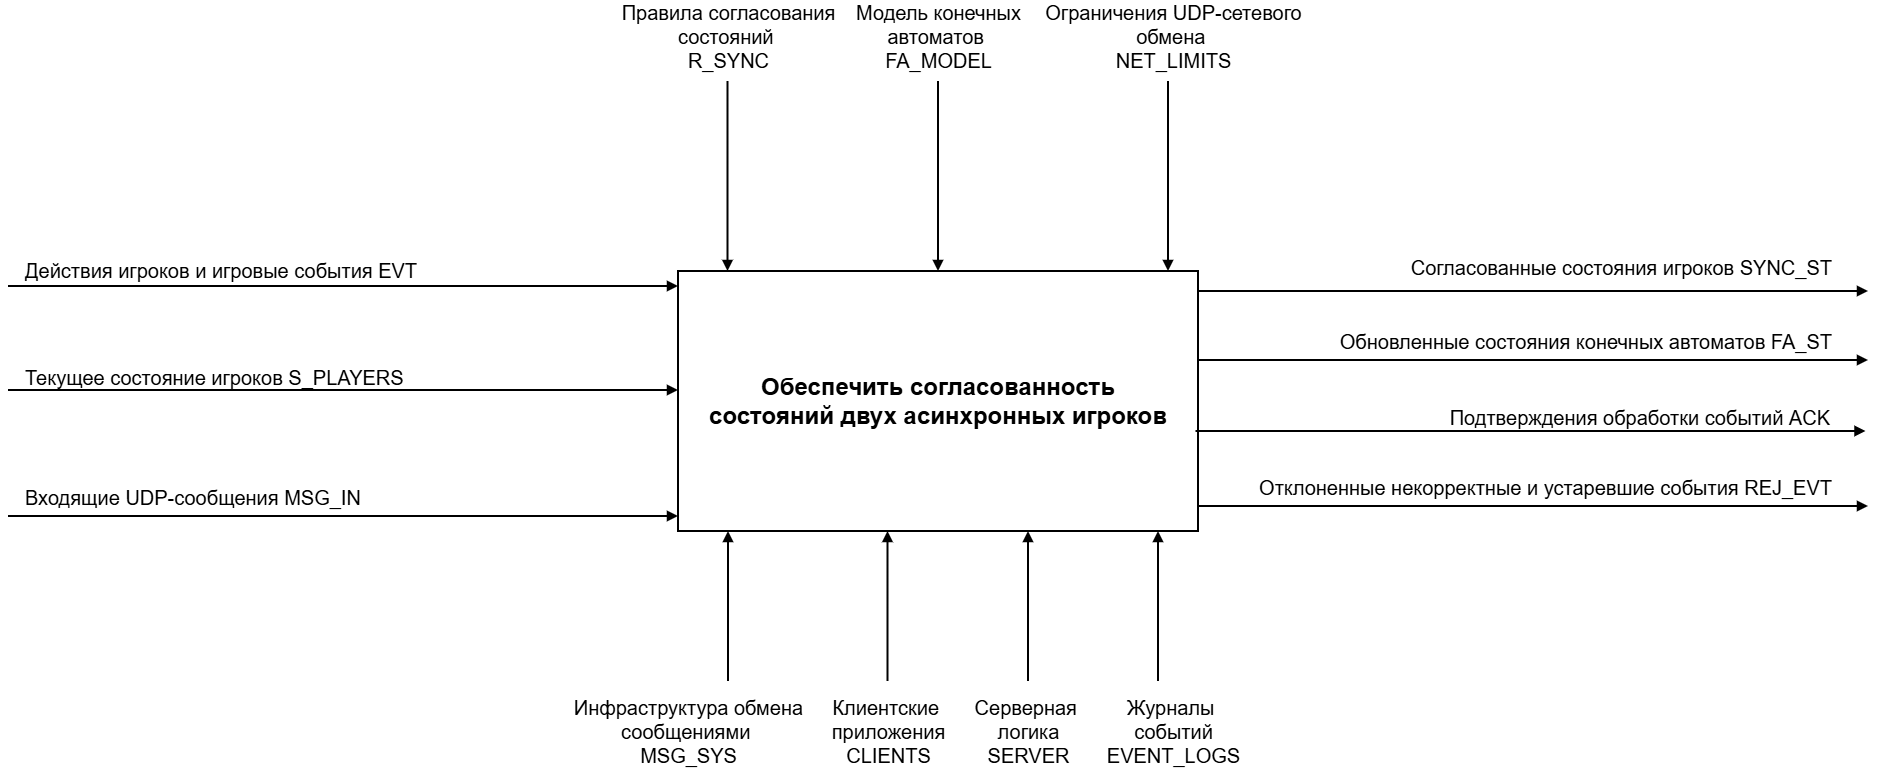
\includegraphics[width=\textwidth]{inc/img/idef0.png}
	\caption{IDEF0-диаграмма постановки задачи обеспечения согласованности состояний}
	\label{img:analysis-idef0-task}
\end{figure}

\subsection{Требования к алгоритмам синхронизации}

Алгоритмы, обеспечивающие согласованность игровых состояний, должны удовлетворять следующим требованиям:
\begin{itemize}
	\item точность --- алгоритм должен обеспечивать минимальные расхождения между состояниями, чтобы игроки наблюдали корректную картину происходящего;
	\item стабильность --- изменения состояния и корректировки должны происходить без резких скачков и визуальных искажений;
	\item устойчивость к сетевым ошибкам --- система должна корректно работать при задержках, потере отдельных пакетов, дублировании и нарушении порядка доставки;
	\item эффективность --- алгоритм не должен перегружать вычислительные ресурсы и должен использовать ограниченный объем сетевого трафика;
	\item проверяемость переходов --- система должна иметь возможность определить, допустимо ли входное событие в текущем состоянии;
	\item воспроизводимость обработки --- одинаковая последовательность событий должна приводить к одинаковому результату на всех участниках взаимодействия.
\end{itemize}

Задача обеспечения согласованности игровых данных формализуется как задача управления состоянием распределенной асинхронной системы, в которой необходимо уравновесить точность, задержку реакции, сетевую нагрузку и корректность обработки событий.

\section{Обзор существующих подходов к синхронизации состояния}

Механизмы синхронизации состояния определяют, каким образом сервер и клиенты обеспечивают актуальность игрового мира, минимизируя расхождения между расчетами на стороне сервера и восприятием игрока. Ниже рассмотрены основные методы, используемые в современных сетевых играх различных жанров.

\subsection{Периодическая репликация состояния}

При использовании снимков сервер с фиксированной частотой отправляет клиентам актуальное состояние мира или его части~\cite{valvesource}. Снимок включает координаты и характеристики активных объектов, состояние игровых сущностей и флаги игровой логики. Этот подход используется в шутерах и других динамичных играх, где важна высокая частота обновления положения объектов и событий~\cite{unity_netcode_docs}.

Преимуществами периодической репликации состояния являются простота реализации и высокая точность согласования при стабильной сети. Клиент регулярно получает авторитетные данные и может восстанавливать свое представление мира даже после потери отдельного обновления.

Недостатками подхода являются высокий объем трафика при большом числе объектов, возможные скачки состояния при применении обновлений и чувствительность к потере последовательных пакетов. Кроме того, передача снимков состояния не описывает причин перехода из одного состояния в другое. Поэтому данный подход хуже подходит для анализа логически значимых событий, которые должны быть применены строго один раз и в определенном порядке.

\subsection{Репликация только изменений}

При репликации изменений сервер отправляет не полный снимок, а только параметры, которые изменились со времени последнего известного клиенту состояния~\cite{unreal_replicate}. Данный метод применяется в системах, где полный снимок мира передавать нецелесообразно из-за большого количества объектов.

Преимуществами метода являются снижение объема передаваемых данных и эффективная работа в больших сценах. Если изменения затрагивают небольшую часть объектов, передача только измененных параметров существенно уменьшает сетевую нагрузку.

К недостаткам относится необходимость хранить предыдущее состояние, относительно которого вычисляется изменение. При потере сообщения клиент может оказаться в состоянии, к которому последующая дельта неприменима. В результате возможно накопление ошибок, поэтому такие системы обычно нуждаются в периодической отправке полного состояния для восстановления согласованности.

\subsection{Событийная модель}

В рамках событийной модели участникам передаются сведения не о полном состоянии объектов, а о произошедших событиях~\cite{GameEventSync2008}. Событие описывает действие, которое должно быть применено к текущему состоянию: начало движения, взаимодействие с объектом, изменение режима, столкновение, создание или уничтожение сущности.

Событийная модель часто используется в RPG, MOBA и стратегиях, где значительная часть взаимодействий описывается дискретными событиями. Преимуществами подхода являются малый объем передаваемых данных, высокая эффективность для логических действий и совместимость с детерминированной симуляцией.

Главная сложность событийной модели заключается в необходимости одинаковой обработки событий на всех сторонах взаимодействия. Если событие потеряно, обработано повторно или применено в неправильном состоянии, локальные представления мира расходятся. Поэтому для событийной синхронизации особенно важны контроль порядка, идентификаторы событий, подтверждения доставки и проверка допустимости переходов.

Данный подход является наиболее близким к теме работы, так как конечный автомат может быть использован для формального описания того, какие события допустимы в каждом состоянии и к каким переходам они приводят.

\subsection{Синхронизация по входным данным}

При синхронизации по входным данным сервер или другой координирующий компонент рассылает клиентам не состояние, а входные команды игроков. Детерминированная симуляция на всех системах должна приводить к одинаковому результату~\cite{photon_sync}.

Этот подход характерен для стратегий в реальном времени, файтингов и симуляторов, где критично поддерживать строгий детерминизм. Преимуществами являются минимальное сетевое потребление и высокая согласованность при условии, что симуляция действительно детерминирована.

Недостатки связаны со сложностью обеспечения детерминизма. Разные процессоры, разные реализации операций с плавающей точкой, отличия в частоте кадров и порядок обновления объектов могут привести к несовпадению результатов. Кроме того, необходимо синхронизировать тики симуляции и очереди входных команд, что повышает сложность реализации.

\subsection{Предсказание состояния на клиенте}

При клиентском предсказании клиент применяет действие игрока немедленно после ввода, не ожидая ответа сервера~\cite{claypool2010latency}. После получения авторитетных данных выполняется проверка и, при необходимости, корректировка состояния.

Механизм предсказания широко используется в динамичных шутерах и экшен-играх, требующих минимальной задержки отклика на ввод игрока. Преимуществами являются высокая отзывчивость управления и снижение субъективного влияния сетевой задержки.

Недостатками являются возможные рывки при корректировке, риск накопления ошибок при нестабильной сети и усложнение логики восстановления состояния. Для логически значимых событий предсказание особенно рискованно, так как ошибка может затронуть не только координаты объекта, но и состояние всей системы взаимодействия.

\subsection{Откат сетевого кода}

Метод отката используется в играх с высокой чувствительностью к синхронизации действий. Клиент предсказывает действия другого участника, а после получения реальных данных выполняется откат состояния и повторный расчет симуляции~\cite{ggpo}. Rollback-подход применяется в аркадных PvP-играх и проектах с высокой чувствительностью к точности столкновений.

Преимуществами метода являются высокая точность взаимодействий и уменьшение видимого влияния сетевой задержки. Недостатками являются повышенная нагрузка на вычислительные ресурсы, необходимость хранить историю состояний и возможные визуальные искажения при пересчете.

Для разрабатываемого метода rollback-подход важен как пример обработки сетевой асинхронности через историю состояний. Однако в рассматриваемой задаче основной акцент делается не на пересчете физической симуляции, а на управлении допустимыми переходами дискретных состояний с помощью конечного автомата.

\section{Обзор методов передачи игровых данных}

\subsection{Надежная и ненадежная доставка данных}

В сетевых играх используются два основных подхода к передаче пакетов: надежная доставка и доставка без гарантий получения~\cite{kurose2013networking}. Они различаются по задержке, стабильности и объему служебной информации.

Надежная доставка, основанная на протоколе TCP, обеспечивает контроль целостности данных и сохраняет порядок передачи пакетов, повторно отправляя утраченные сегменты~\cite{stevens2011tcpip}. Такая модель удобна для передачи данных, потеря которых недопустима. Однако TCP добавляет задержку из-за механизма подтверждений, повторных передач и сохранения общего порядка байтового потока. Для динамичных игр с высокой частотой обновления состояния это может приводить к задержке обработки новых данных из-за ожидания восстановления старых сегментов.

Ненадежная доставка, реализованная через протокол UDP, не гарантирует получение каждого отдельного пакета, но обеспечивает меньшие накладные расходы и минимально возможную задержку. Большинство сетевых игр используют UDP и собственные механизмы надежности для критичных данных. Такой подход позволяет выбирать, какие сообщения требуют подтверждения и повторной отправки, а какие могут быть потеряны без нарушения логики.

Для разрабатываемого метода использование UDP означает, что контроль доставки, порядка и дублирования логически значимых событий должен выполняться на прикладном уровне. Это соответствует событийной природе метода: не все данные требуют надежной передачи, но события, приводящие к переходам конечного автомата, должны быть обработаны согласованно.

\subsection{Классификация и приоритизация игровых пакетов}

Игровые данные по-разному реагируют на задержки и потери, поэтому пакеты обычно разделяют на классы приоритетности. Это позволяет оптимизировать передачу и избежать перегрузки канала связи.

Критичные данные включают команды игрока, результаты столкновений и важные события игровой логики. Они должны доставляться максимально быстро и целостно, поскольку их потеря может привести к заметной рассинхронизации состояния.

Важные, но допускающие потерю данные могут передаваться чаще, но без гарантии получения. Потеря части таких пакетов компенсируется новыми обновлениями в следующих сообщениях. Примером являются часто обновляемые координаты объектов, когда более новое значение делает устаревшее сообщение неактуальным.

Второстепенные данные, например визуальные эффекты, косметические параметры и отдельные звуковые события, могут передаваться с низким приоритетом или не передаваться вовсе, если клиент способен корректно воспроизводить их локально.

В контексте данной работы к критичным данным относятся события, изменяющие состояние конечного автомата. Такие события должны иметь идентификатор, номер последовательности и признак подтверждения, чтобы принимающая сторона могла обнаружить потерю, повтор или нарушение порядка.

\subsection{Механизмы обеспечения частичной надежности}

Поскольку UDP сам по себе не предоставляет гарантированную доставку, игровые движки внедряют дополнительные механизмы частичной надежности, позволяющие гарантировать передачу важных данных без превращения всего обмена в аналог TCP.

К таким механизмам относятся:
\begin{itemize}
	\item подтверждение доставки для отдельных типов пакетов;
	\item повторная отправка важных данных при отсутствии подтверждения;
	\item нумерация пакетов для восстановления порядка исполнения команд;
	\item фильтрация дубликатов по идентификаторам сообщений;
	\item отбрасывание устаревших сообщений, которые относятся к уже пройденному состоянию системы.
\end{itemize}

Эти механизмы позволяют экономно расходовать сетевой ресурс, сохраняя критичные данные в актуальном состоянии. При этом важно, чтобы повторная отправка не приводила к повторному применению одного и того же события. Поэтому прикладный уровень должен различать доставку сообщения и применение события к состоянию системы.

\subsection{Адаптивные алгоритмы передачи данных}

Современные сетевые игры используют динамические методы, которые подстраиваются под качество канала. Адаптивные алгоритмы позволяют снижать нагрузку в условиях высокой задержки или потери пакетов и увеличивать точность передачи при стабильном соединении.

К распространенным техникам относятся:
\begin{itemize}
	\item изменение частоты отправки пакетов в зависимости от текущей задержки;
	\item снижение точности квантования при перегрузке сети;
	\item динамическое отключение второстепенных данных;
	\item регулирование частоты отправки обновлений в зависимости от важности объектов.
\end{itemize}

Такие методы повышают устойчивость сетевой игры при различных условиях соединения и снижают риск возникновения рассинхронизации. Однако они не заменяют механизмы согласования событий. Если логически значимое событие потеряно или обработано в неверном состоянии, уменьшение частоты передачи второстепенных данных не восстановит корректность системы.

\section{Типовые игровые данные, подлежащие хранению, обновлению и передаче}

В процессе работы многопользовательского игрового приложения сервер и клиенты обмениваются различными типами данных, описывающих состояние объектов, игровые события и вспомогательные параметры~\cite{gregory2018gamedev}. Эти данные определяют внутреннюю логику игрового мира и корректность взаимодействия игроков.

\subsection{Данные состояния объектов}

Состояние объектов описывает характеристики сущностей и является основой игрового мира. Эти данные подлежат частому обновлению.

К типичным данным состояния объектов относятся:
\begin{itemize}
	\item позиция объекта;
	\item скорость и направление движения;
	\item поворот и ориентация;
	\item состояние анимации;
	\item физические параметры.
\end{itemize}

Эти данные требуют высокой точности и частой синхронизации. Особенно это критично для FPS, гонок и экшен-игр, где любое отклонение в позиции приводит к заметным ошибкам восприятия. В то же время часть таких данных может устаревать: если новое значение позиции уже получено, старое значение обычно не требуется применять.

\subsection{Данные игровой логики}

Помимо визуального состояния объектов существуют параметры, влияющие на игровую логику.

В эту категорию входят:
\begin{itemize}
	\item здоровье;
	\item ресурсы;
	\item активные эффекты;
	\item флаги состояний;
	\item текущая фаза взаимодействия.
\end{itemize}

Данные игровой логики обновляются реже, чем параметры движения, но требуют более надежной доставки. Ошибка в таких данных приводит к различию в результатах игровых событий. Например, если один участник считает, что действие уже завершено, а другой продолжает считать его активным, то последующие события будут интерпретированы по-разному.

\subsection{Данные взаимодействия и событий}

Игровые события отображают дискретные изменения состояния мира. Они могут быть результатом действий игрока или следствием внутренних механик.

Примеры событий:
\begin{itemize}
	\item совершение действия;
	\item взаимодействие с объектом;
	\item создание или уничтожение объекта;
	\item начало или завершение игровой фазы;
	\item срабатывание триггера.
\end{itemize}

События требуют надежной обработки, поскольку их потеря приводит к расхождениям в симуляции между игроками. Кроме того, событие должно применяться в определенном состоянии системы. Если событие доставлено позже, чем система перешла в следующее состояние, оно может стать устаревшим и должно быть обработано особым образом.

Именно данные взаимодействия и событий являются основным объектом рассмотрения в разрабатываемом методе. Для них необходимо обеспечить доставку, порядок, защиту от повторного применения и проверку допустимости перехода.

\subsection{Вспомогательные данные}

Некоторые игры используют дополнительные данные, не относящиеся напрямую к состоянию объектов, но влияющие на корректность симуляции.

К таким данным относятся:
\begin{itemize}
	\item навигационные сетки;
	\item вспомогательные маркеры;
	\item данные о временных параметрах;
	\item параметры конфигурации игровой сессии.
\end{itemize}

Эти данные чаще хранятся на сервере и передаются клиенту при необходимости. Их изменение обычно происходит реже, чем изменение состояния объектов, однако несогласованность таких данных может привести к разному поведению симуляции на разных сторонах.

\subsection{Визуальные данные}

Некоторые данные не влияют на игровую логику напрямую и могут синхронизироваться реже или генерироваться на клиенте без участия сервера.

К таким данным относятся:
\begin{itemize}
	\item эффекты частиц;
	\item косметические параметры;
	\item звуковые события;
	\item вспомогательные элементы интерфейса.
\end{itemize}

Передача таких данных оптимизируется в первую очередь при ограничении пропускной способности. Потеря визуального события может ухудшить восприятие, но обычно не приводит к нарушению логики взаимодействия.

\subsection{Метаданные и технические данные}

Помимо игровых данных существует набор технической информации, обеспечивающей корректную работу сетевого взаимодействия.

К ним относятся:
\begin{itemize}
	\item идентификаторы объектов;
	\item временные метки;
	\item номера последовательности;
	\item контрольные суммы;
	\item служебные флаги;
	\item идентификаторы подтверждений доставки.
\end{itemize}

Такие данные не видны игроку, но они важны для поддержания согласованности состояния и предотвращения ошибок. В методе, основанном на конечных автоматах, технические данные используются для связи сетевого сообщения с конкретным событием, состоянием автомата и фактом обработки этого события.

\section{Основные причины возникновения рассинхронизации}

Рассинхронизация состояния --- это расхождение между данными, хранящимися на авторитетной стороне, и состоянием, которое отображается или обрабатывается в клиентских приложениях. Возникновение рассинхронизации обусловлено как особенностями сетевого окружения, так и архитектурными проблемами внутри игрового приложения.

\subsection{Сетевые задержки}

Одной из наиболее распространенных причин рассинхронизации является задержка передачи данных~\cite{pantel2002lag}. Игровой клиент всегда получает состояние с определенной задержкой, зависящей от качества соединения. Если задержка непостоянна и резко меняется, клиент может получить обновления позже или раньше ожидаемого момента, что вызывает временные расхождения в позициях объектов и фазах событий.

Ситуация ухудшается в условиях нестабильных сетей, где вариативность задержек возрастает. Для событийной синхронизации это означает, что событие, созданное раньше, может быть доставлено позже события, созданного после него. Без контроля порядка такая ситуация приводит к некорректной последовательности переходов состояния.

\subsection{Потеря, дублирование и нарушение порядка доставки пакетов}

При использовании ненадежных протоколов часть пакетов может теряться или приходить в другом порядке. Это приводит к следующим ошибкам:
\begin{itemize}
	\item объект остается на устаревшей позиции;
	\item проигрываются неактуальные события;
	\item происходит откат состояния назад;
	\item одно и то же событие применяется несколько раз;
	\item переход состояния выполняется без необходимого предшествующего события.
\end{itemize}

Хотя игровые движки реализуют механизмы частичной надежности, абсолютной защиты от подобных проблем нет. Поэтому прикладная логика должна быть готова к получению некорректных, повторных и устаревших сообщений.

\subsection{Недетерминизм симуляции}

Некоторые игры опираются на локальный расчет физики или игровой логики на стороне клиента. Любое незначительное отличие в вычислениях может привести к расхождению состояния. Основные источники недетерминизма:
\begin{itemize}
	\item использование чисел с плавающей точкой, дающих разные результаты на разных процессорах;
	\item различный порядок обновления объектов на разных клиентах;
	\item вариации частоты кадров, влияющие на расчет физики.
\end{itemize}

Такие проблемы особенно заметны в стратегиях и симуляторах, где большое количество объектов должно развиваться по одинаковым правилам в течение длительного времени. В задачах с конечными автоматами недетерминизм проявляется как неодинаковое выполнение переходов при одинаковых входных событиях, что делает систему непредсказуемой.

\subsection{Различия в производительности клиентских устройств}

Игровые клиенты могут работать с разной скоростью в зависимости от мощности процессора, видеокарты и текущей нагрузки. Если частота обновления симуляции отличается, одни клиенты рассчитывают больше физических шагов, чем другие, а предсказания состояния расходятся с авторитетной логикой.

В играх, где симуляция сильно зависит от стабильной частоты кадров, такие различия являются источником ошибок. Для снижения влияния этого фактора часто используется фиксированный шаг симуляции, синхронизация тиков и отделение логического состояния от частоты отрисовки.

\subsection{Неправильная или неполная сериализация данных}

При передаче состояния объекты сериализуются. Ошибки сериализации приводят к тому, что данные не совпадают на клиенте и сервере. Это может быть вызвано:
\begin{itemize}
	\item пропуском некоторых параметров объекта;
	\item отправкой данных в неправильном формате;
	\item несогласованностью типов при чтении и записи;
	\item различием версий протокола обмена.
\end{itemize}

Для событийной модели ошибка сериализации особенно опасна, если затрагивает идентификатор события, номер последовательности, тип события или состояние, к которому оно относится. В этом случае сообщение может быть доставлено, но обработано как другое событие или как событие для другого состояния.

\subsection{Несогласованный порядок выполнения событий}

Если события обрабатываются не в том же порядке, что на авторитетной стороне, результаты симуляции расходятся. Это происходит из-за локальных оптимизаций клиента, попадания пакетов с разными временными метками, параллельного выполнения задач и применения предсказания до получения подтверждения от сервера.

Несогласованная обработка событий особенно критична для игр с динамичными механиками взаимодействия. Например, если событие завершения действия обработано раньше события его начала, система может перейти в недопустимое состояние. Поэтому порядок событий должен контролироваться не только на транспортном уровне, но и на уровне модели состояний.

\subsection{Ошибки в предсказании и последующей коррекции состояния}

Клиентское предсказание значительно повышает отзывчивость, но несет риск ошибок. Предсказание может расходиться с реальными данными сервера, что приводит к резким скачкам при корректировке, неверным расчетам следующего состояния и накоплению ошибки при плохой связи~\cite{gamenetpatterns}.

Такие проблемы заметны при нестабильной задержке сети и большом количестве корректировок. В дискретной логике взаимодействия ошибка предсказания может привести к тому, что клиент временно перейдет в состояние, которое затем будет отклонено авторитетной стороной. В этом случае система должна иметь способ безопасно отменить или скорректировать переход.

\section*{Вывод}

В данном разделе была рассмотрена предметная область синхронизации игровых состояний в многопользовательских приложениях. 
Было показано, что такие приложения являются распределенными асинхронными системами, в которых рассинхронизация может возникать из-за задержек, потерь пакетов, нарушения порядка доставки, 
недетерминизма симуляции и неодинаковой обработки событий.

Была формализована задача обеспечения согласованности игровых данных. Состояние игрового мира представлено как совокупность состояний сущностей, изменяемых под воздействием входных команд и событий. 
Рассогласование состояния определено через различие параметров сущностей и логических состояний системы.

\chapter{Конструкторский раздел}\label{design}

\section{Требования к разрабатываемому методу}

Разрабатываемый метод должен обеспечивать согласованную обработку логически значимых игровых событий в условиях асинхронного сетевого обмена. 
Под логически значимым событием понимается событие, приводящее к изменению состояния игрока, общего игрового объекта или состояния взаимодействия между двумя игроками.

К методу синхронизации предъявляются следующие требования:
\begin{itemize}
	\item метод должен описывать взаимодействие двух игроков как обработку событий, вызывающих допустимые переходы конечного автомата синхронизируемого объекта;
	\item обработка критичных событий должна выполняться через авторитетный сервер, проверяющий порядок сообщений и допустимость применения события;
	\item каждое событие, изменяющее состояние системы, должно иметь уникальный идентификатор;
	\item каждое событие должно иметь номер последовательности в потоке событий игрока-отправителя;
	\item повторное получение одного и того же события не должно приводить к повторному изменению состояния;
	\item потеря события или подтверждения должна обнаруживаться на прикладном уровне;
	\item неподтвержденные события должны повторно отправляться до получения подтверждения;
	\item события, недопустимые для целевого конечного автомата, должны отклоняться;
	\item метод должен учитывать возможность задержки, потери, дублирования и нарушения порядка доставки UDP-пакетов.
\end{itemize}

Ограничением метода является рассмотрение взаимодействия двух игроков. Такое ограничение позволяет явно описать события и состояния игровых объектов, 
не вводя дополнительные механизмы масштабирования.

\section{Функциональная модель метода}

Разрабатываемый метод использует клиент-серверную схему обмена. Клиент формирует событие по локальному действию игрока и отправляет его серверу по UDP. 
Сервер выступает авторитетной стороной. Он проверяет событие, применяет его к целевому конечному автомату, отправляет подтверждение игроку-отправителю и рассылает подтвержденное событие клиентам.

Метод синхронизации включает следующие основные этапы:
\begin{enumerate}
	\item формирование локального игрового события на стороне клиента;
	\item присвоение событию идентификатора и номера последовательности;
	\item отправка события серверу;
	\item сохранение события в журнале неподтвержденных событий клиента;
	\item получение события сервером;
	\item проверка идентификатора события и фильтрация дубликатов;
	\item проверка номера последовательности события;
	\item поиск целевого объекта по идентификатору;
	\item применение события к конечному автомату целевого объекта;
	\item отправка подтверждения клиенту-отправителю;
	\item рассылка подтвержденного события клиентам;
	\item удаление подтвержденного события из журнала неподтвержденных событий клиента.
\end{enumerate}


Декомпозиция функции обеспечения согласованности состояний приведена на рисунке~\ref{img:design-idef0}. 
Она отражает последовательность обработки события от формирования на стороне клиента до подтверждения обработки и распространения результата.

\begin{figure}[H]
	\centering
	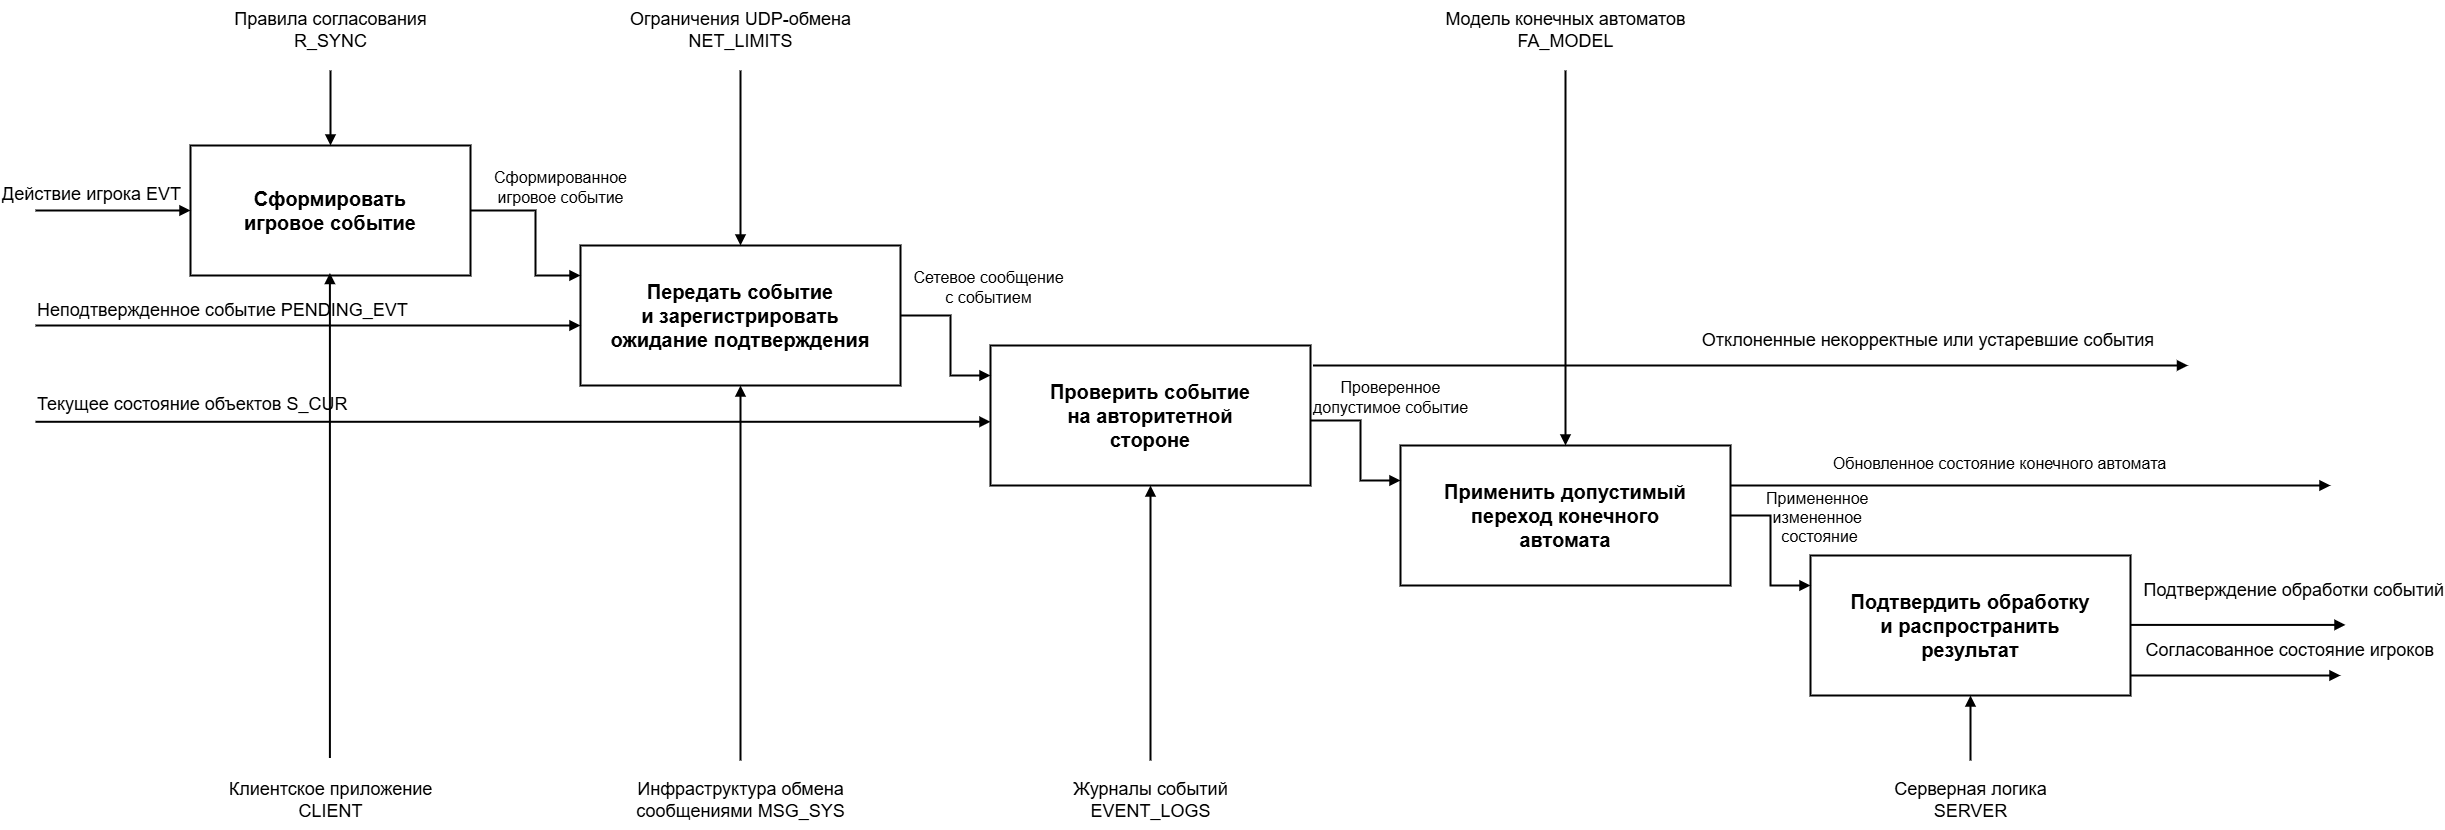
\includegraphics[width=\textwidth]{inc/img/idef1.png}
	\caption{IDEF0-диаграмма метода обеспечения согласованности состояний}
	\label{img:design-idef0}
\end{figure}

\section{Формальная модель синхронизации}

Состояние системы двух игроков в момент времени $t$ зададим как:
\[
	S(t) = \left(S_1(t), S_2(t), O(t), N(t)\right),
\]
где:
\begin{itemize}
	\item $S_1(t)$ --- локальное состояние первого игрока;
	\item $S_2(t)$ --- локальное состояние второго игрока;
	\item $O(t)$ --- множество состояний синхронизируемых игровых объектов;
	\item $N(t)$ --- состояние сетевого протокола синхронизации.
\end{itemize}

Множество синхронизируемых игровых объектов зададим как:
\[
	O = \{o_1, o_2, \ldots, o_n\}.
\]
Каждый объект $o_j$ имеет идентификатор $id(o_j)$ и конечный автомат:
\[
	A_j = \left(Q_j, E_j, \delta_j, q_j^0\right),
\]
где:
\begin{itemize}
	\item $Q_j$ --- множество состояний объекта;
	\item $E_j$ --- множество допустимых событий объекта;
	\item $\delta_j$ --- функция переходов;
	\item $q_j^0$ --- начальное состояние.
\end{itemize}

Игровое событие зададим кортежем:
\[
	e_k = \left(eventId_k, sequence_k, playerId_k, sourceObject_k, targetObject_k, type_k\right),
\]
где:
\begin{itemize}
	\item $eventId_k$ --- уникальный идентификатор события;
	\item $sequence_k$ --- номер события в потоке игрока-отправителя;
	\item $playerId_k$ --- идентификатор игрока-отправителя;
	\item $sourceObject_k$ --- идентификатор объекта-источника;
	\item $targetObject_k$ --- идентификатор целевого объекта;
	\item $type_k$ --- тип события.
\end{itemize}

Сетевое сообщение, передаваемое по UDP, зададим кортежем:
\[
	m_k = \left(messageType_k, event_k, ackId_k, senderId_k, targetId_k\right),
\]
где:
\begin{itemize}
	\item $messageType_k$ --- тип сетевого сообщения;
	\item $event_k$ --- игровое событие;
	\item $ackId_k$ --- идентификатор подтверждаемого события;
	\item $senderId_k$ --- идентификатор отправителя сообщения;
	\item $targetId_k$ --- идентификатор получателя подтверждения.
\end{itemize}

В методе используются три типа сетевых сообщений:
\begin{itemize}
	\item \texttt{ClientHello} --- служебное сообщение регистрации клиента;
	\item \texttt{PuzzleEvent} --- сообщение, содержащее игровое событие;
	\item \texttt{Acknowledgement} --- подтверждение обработки события.
\end{itemize}

Состояние протокола синхронизации на стороне клиента можно представить кортежем:
\[
	N_c = \left(id_c, seq_c^{out}, L_c, A_c\right),
\]
где:
\begin{itemize}
	\item $id_c$ --- идентификатор клиента;
	\item $seq_c^{out}$ --- номер следующего исходящего события;
	\item $L_c$ --- журнал отправленных, но не подтвержденных событий;
	\item $A_c$ --- множество уже примененных событий.
\end{itemize}

Состояние протокола синхронизации на стороне сервера можно представить кортежем:
\[
	N_s = \left(R_s, A_s, H_s\right),
\]
где:
\begin{itemize}
	\item $R_s$ --- множество зарегистрированных конечных автоматов игровых объектов;
	\item $A_s$ --- множество уже примененных событий;
	\item $H_s$ --- отображение идентификатора игрока в номер следующего ожидаемого события.
\end{itemize}

Применение события к игровому объекту определяется функцией:
\[
	Apply(e_k, o_j) =
	\begin{cases}
		true, & \text{если } type_k \in E_j \text{ и переход } \delta_j \text{ допустим};\\
		false, & \text{если событие не может быть применено к объекту}.
	\end{cases}
\]

В таком представлении сетевой уровень передает события, менеджер синхронизации проверяет идентификаторы и порядок сообщений, а допустимость перехода определяется целевым объектом, реализующим конечный автомат.

\section{Состояния протокола синхронизации}

Для описания работы метода выделим следующие состояния протокола синхронизации:
\begin{itemize}
	\item $q_0$ --- регистрация клиента;
	\item $q_1$ --- ожидание локального или сетевого события;
	\item $q_2$ --- формирование исходящего события;
	\item $q_3$ --- ожидание подтверждения;
	\item $q_4$ --- обработка события на сервере;
	\item $q_5$ --- рассылка подтвержденного события;
	\item $q_6$ --- применение подтвержденного события на клиенте;
	\item $q_7$ --- повторная отправка неподтвержденного события;
	\item $q_8$ --- отклонение события.
\end{itemize}

Состояние $q_0$ используется при запуске клиента. Клиент отправляет серверу сообщение \texttt{ClientHello}, содержащее идентификатор игрока. Сервер сохраняет сетевой адрес клиента для последующей рассылки сообщений.

Состояние $q_1$ соответствует обычному режиму работы, в котором клиент ожидает локального действия игрока или входящего сетевого сообщения.

Состояние $q_2$ возникает при локальном действии игрока. Действие преобразуется в событие, которому присваиваются идентификатор и номер последовательности.

Состояние $q_3$ используется после отправки критичного события серверу. Клиент хранит событие в журнале неподтвержденных событий и ожидает подтверждения.

Состояние $q_4$ соответствует обработке события сервером. Сервер проверяет дубликаты, номер последовательности, наличие целевого объекта и допустимость применения события к конечному автомату.

Состояние $q_5$ используется после успешного применения события сервером. Сервер отправляет подтверждение игроку-отправителю и рассылает подтвержденное событие клиентам.

Состояние $q_6$ соответствует обработке подтвержденного события клиентом. Клиент применяет событие к локальному конечному автомату целевого объекта, если событие еще не было обработано.

Состояние $q_7$ возникает при истечении времени ожидания подтверждения. Клиент повторно отправляет событие с теми же значениями идентификатора и номера последовательности.

Состояние $q_8$ используется при получении дубликата, устаревшего события, события с нарушенным порядком или события, которое не может быть применено к целевому конечному автомату.

\begin{figure}[H]
	\centering
	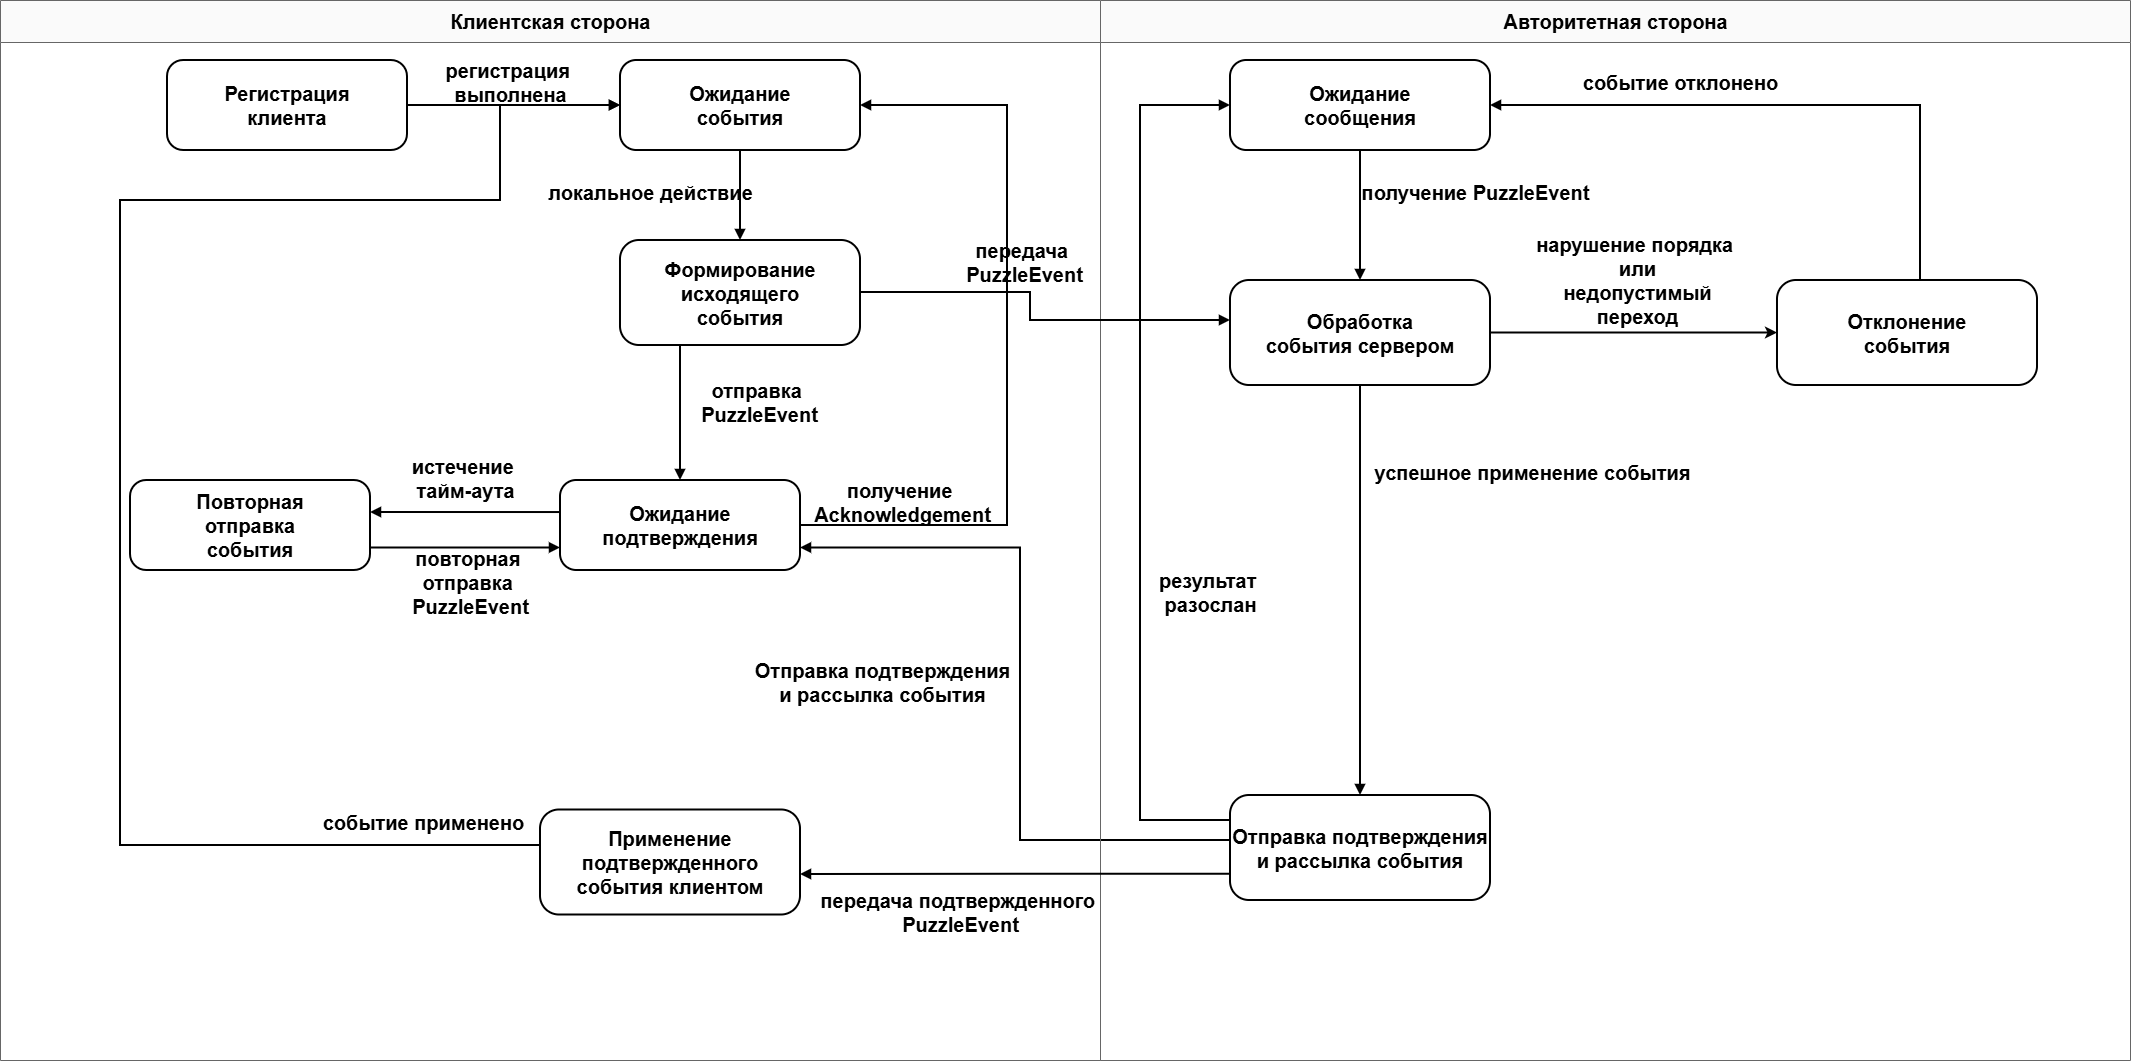
\includegraphics[width=\textwidth]{inc/img/diagram_sync.png}
	\caption{Диаграмма состояний протокола синхронизации}
	\label{img:design-state-machine}
\end{figure}

\section{Модель переходов протокола синхронизации}

Основные переходы протокола синхронизации приведены в таблице~\ref{tab:fsm-transitions}.

{
	\renewcommand{\arraystretch}{1.2}
	\begin{longtable}{|p{3.4cm}|p{4.3cm}|p{3.7cm}|p{3cm}|}
		\caption{Основные переходы протокола синхронизации}
		\label{tab:fsm-transitions}\\
		\hline
		Текущее состояние & Событие & Условие & Следующее состояние \\ \hline
		\endfirsthead
		\hline
		Текущее состояние & Событие & Условие & Следующее состояние \\ \hline
		\endhead
		Регистрация клиента & Отправлен \texttt{ClientHello} & Клиент имеет идентификатор & Ожидание события \\ \hline
		Ожидание события & Локальное действие игрока & Сформирован тип события & Формирование исходящего события \\ \hline
		Формирование исходящего события & Событие отправлено серверу & Событие сохранено в журнале & Ожидание подтверждения \\ \hline
		Ожидание подтверждения & Получен \texttt{Acknowledgement} & Идентификатор события совпадает & Ожидание события \\ \hline
		Ожидание подтверждения & Истек тайм-аут & Событие остается в журнале & Повторная отправка \\ \hline
		Повторная отправка & Событие отправлено повторно & Идентификатор и номер не изменены & Ожидание подтверждения \\ \hline
		Ожидание события & Получен \texttt{PuzzleEvent} сервером & Номер события ожидаемый & Обработка события сервером \\ \hline
		Обработка события сервером & Событие применено к FSM & Переход допустим & Рассылка подтвержденного события \\ \hline
		Обработка события сервером & Событие является дубликатом & Ключ события уже обработан & Отклонение события \\ \hline
		Обработка события сервером & Нарушен порядок & Номер больше ожидаемого & Отклонение события \\ \hline
		\pagebreak
		Рассылка подтвержденного события & Событие отправлено клиентам & Событие принято сервером & Ожидание события \\ \hline
		Ожидание события & Получено подтвержденное событие клиентом & Событие не обработано ранее & Применение события клиентом \\ \hline
		Применение события клиентом & Событие применено к FSM & Переход допустим & Ожидание события \\ \hline
	\end{longtable}
}

Дубликат события не должен приводить к повторному переходу конечного автомата. Если ключ события уже содержится во множестве обработанных событий, состояние объекта не изменяется. На сервере при получении повторного события дополнительно отправляется подтверждение игроку-отправителю, поскольку повтор мог возникнуть из-за потери предыдущего подтверждения.

Если сервер получает событие с номером последовательности меньше ожидаемого, оно рассматривается как устаревшее. Если номер больше ожидаемого, событие не применяется, так как перед ним должно быть обработано одно или несколько предыдущих событий. Такое сообщение не подтверждается, что приводит к повторной отправке со стороны клиента до восстановления корректного порядка доставки.

\section{Структура передаваемых событий}

Передаваемые сообщения делятся на служебные сообщения регистрации, игровые события и подтверждения. Игровые события изменяют состояние конечного автомата целевого игрового объекта. Подтверждения используются для удаления события из журнала неподтвержденных событий клиента.

К игровым событиям относятся:
\begin{itemize}
	\item нажатие интерактивной кнопки;
	\item нажатие или отпускание нажимной плиты;
	\item переключение рычага;
	\item активация моста;
	\item нажатие цветной кнопки;
	\item завершение игровой задачи.
\end{itemize}

Структура игрового события должна включать поля, необходимые для маршрутизации события, контроля порядка и защиты от повторной обработки. В таблице~\ref{tab:event-fields} приведен набор полей события.

\begin{table}[H]
	\caption{Структура игрового события}
	\label{tab:event-fields}
	\centering
	\renewcommand{\arraystretch}{1.2}
	\begin{tabular}{|p{4.5cm}|p{9.5cm}|}
		\hline
		Поле & Назначение \\ \hline
		\texttt{eventId} & Уникальный идентификатор события \\ \hline
		\texttt{sequenceNumber} & Номер события в потоке игрока-отправителя \\ \hline
		\texttt{sourcePlayerId} & Идентификатор игрока-отправителя \\ \hline
		\texttt{sourceObjectId} & Идентификатор объекта, сформировавшего событие \\ \hline
		\texttt{targetObjectId} & Идентификатор объекта, к которому должно быть применено событие \\ \hline
		\texttt{eventType} & Тип игрового события \\ \hline
	\end{tabular}
\end{table}

Структура сетевого сообщения приведена в таблице~\ref{tab:message-fields}.

\begin{table}[H]
	\caption{Структура сетевого сообщения}
	\label{tab:message-fields}
	\centering
	\renewcommand{\arraystretch}{1.2}
	\begin{tabular}{|p{4.5cm}|p{9.5cm}|}
		\hline
		Поле & Назначение \\ \hline
		\texttt{messageType} & Тип сетевого сообщения: \texttt{ClientHello}, \texttt{PuzzleEvent} или \texttt{Acknowledgement} \\ \hline
		\texttt{puzzleEvent} & Игровое событие, передаваемое в сообщении типа \texttt{PuzzleEvent} \\ \hline
		\texttt{ackForEventId} & Идентификатор подтверждаемого события \\ \hline
		\texttt{senderPlayerId} & Идентификатор отправителя сообщения \\ \hline
		\texttt{targetPlayerId} & Идентификатор клиента, которому адресовано подтверждение \\ \hline
	\end{tabular}
\end{table}

Поле \texttt{sequenceNumber} используется для контроля порядка, а поле \texttt{eventId} вместе с \texttt{sourcePlayerId} --- для фильтрации дубликатов. Допустимость перехода не передается в сообщении явно, 
она определяется целевым объектом при вызове метода применения события.


\section{Механизм подтверждения и повторной отправки}

Так как UDP не гарантирует доставку сообщений, надежность для критичных событий обеспечивается на прикладном уровне. После отправки события клиент помещает его в журнал неподтвержденных событий $L_c$. В журнале событие хранится по идентификатору \texttt{eventId}.

Сервер после успешной проверки и применения события отправляет подтверждение. Подтверждение содержит идентификатор принятого события и идентификатор клиента, которому оно адресовано. После получения подтверждения клиент удаляет событие из журнала неподтвержденных событий.

Если подтверждение не получено за время $T_{ack}$, клиент повторно отправляет событие. Повторная отправка не создает новое событие, а использует тот же идентификатор и тот же номер последовательности. Благодаря этому сервер может отличить повторную отправку от нового игрового события.
В разработанном методе повторная отправка продолжается, пока событие находится в журнале неподтвержденных событий.

Последовательность обмена сообщениями в обоих случаях определяется состояниями протокола. После отправки \texttt{PuzzleEvent} клиент переходит в ожидание подтверждения, сервер выполняет авторитетную проверку события, а при отсутствии подтверждения клиент повторно отправляет тот же экземпляр события.

\section{Контроль порядка сообщений}

Для каждого игрока сервер поддерживает номер следующего ожидаемого события. Клиент увеличивает номер последовательности при создании нового логически значимого события. Сервер сравнивает полученный номер с ожидаемым значением.

При получении события возможны следующие случаи:
\begin{itemize}
	\item номер события равен ожидаемому --- событие может быть проверено и применено;
	\item номер события меньше ожидаемого --- событие считается устаревшим или повторным;
	\item номер события больше ожидаемого --- одно или несколько предыдущих событий отсутствуют, поэтому текущее событие не применяется.
\end{itemize}

Для двух игроков достаточно хранить по одному счетчику ожидаемого события на каждого игрока. Это упрощает реализацию по сравнению с системами, где требуется поддерживать множество потоков событий от большого числа участников.

Если событие с большим номером последовательности приходит раньше предыдущих событий, сервер не применяет его и не отправляет подтверждение. Клиент продолжает повторную отправку неподтвержденного события, что позволяет восстановить обработку после доставки недостающего сообщения.

\section{Алгоритм синхронизации состояний}

Схемы алгоритмов обработки исходящего события, серверной обработки события и повторной отправки приведены на рисунках~\ref{img:design-outgoing-event}--\ref{img:design-resend}.

\begin{figure}[H]
	\centering
	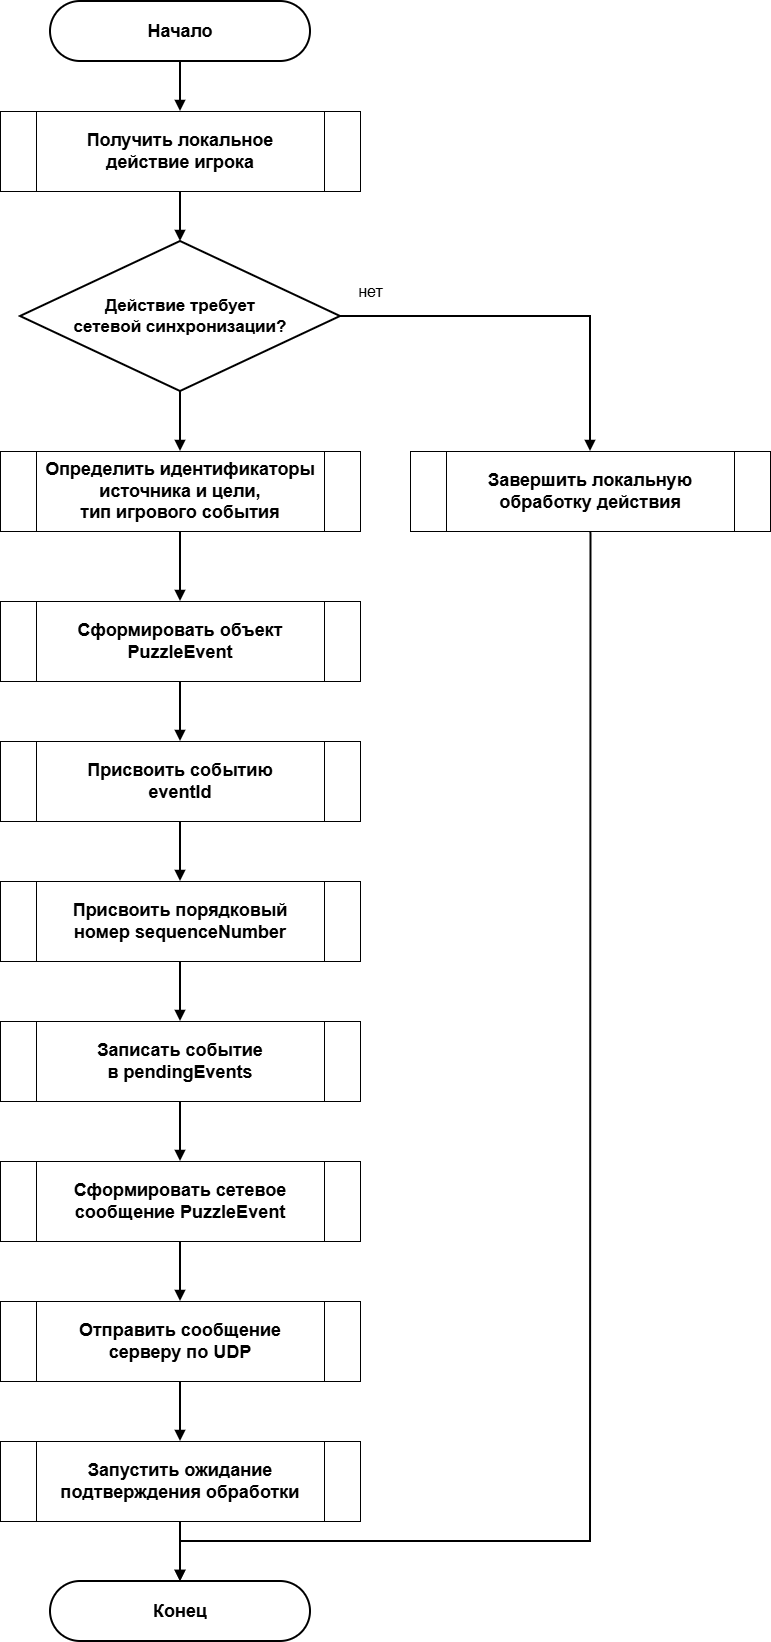
\includegraphics[height=0.82\textheight]{inc/img/outcomming_event.png}
	\caption{Схема алгоритма обработки исходящего события}
	\label{img:design-outgoing-event}
\end{figure}

\begin{figure}[H]
	\centering
	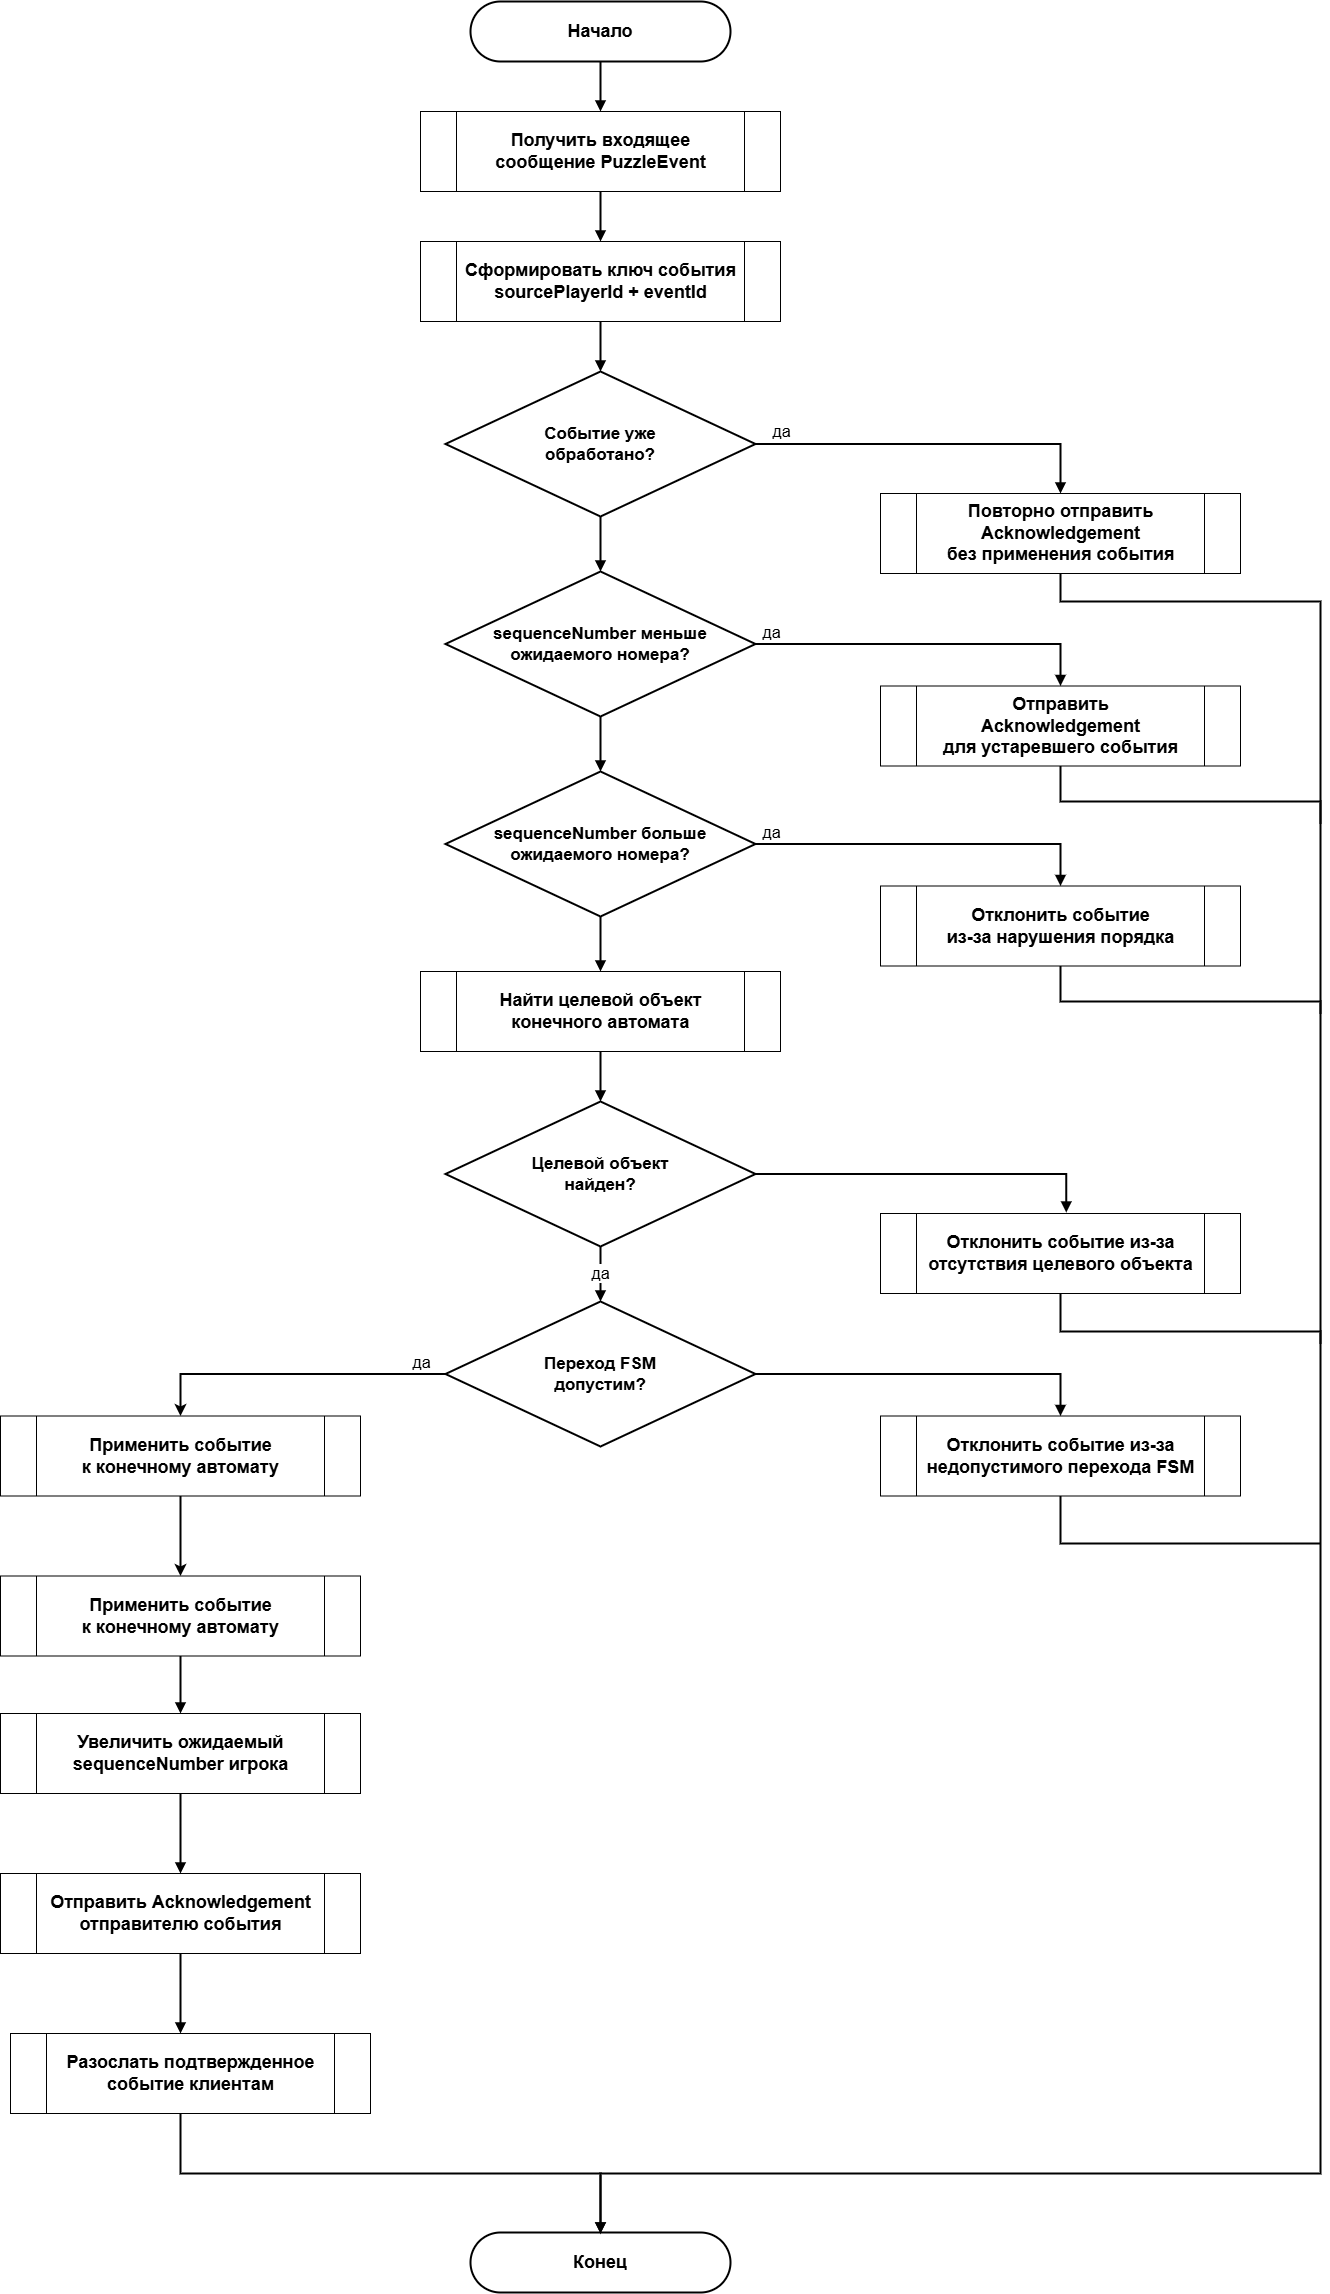
\includegraphics[height=0.82\textheight]{inc/img/server_event.png}
	\caption{Схема алгоритма обработки события сервером}
	\label{img:design-incoming-event}
\end{figure}

\begin{figure}[H]
	\centering
	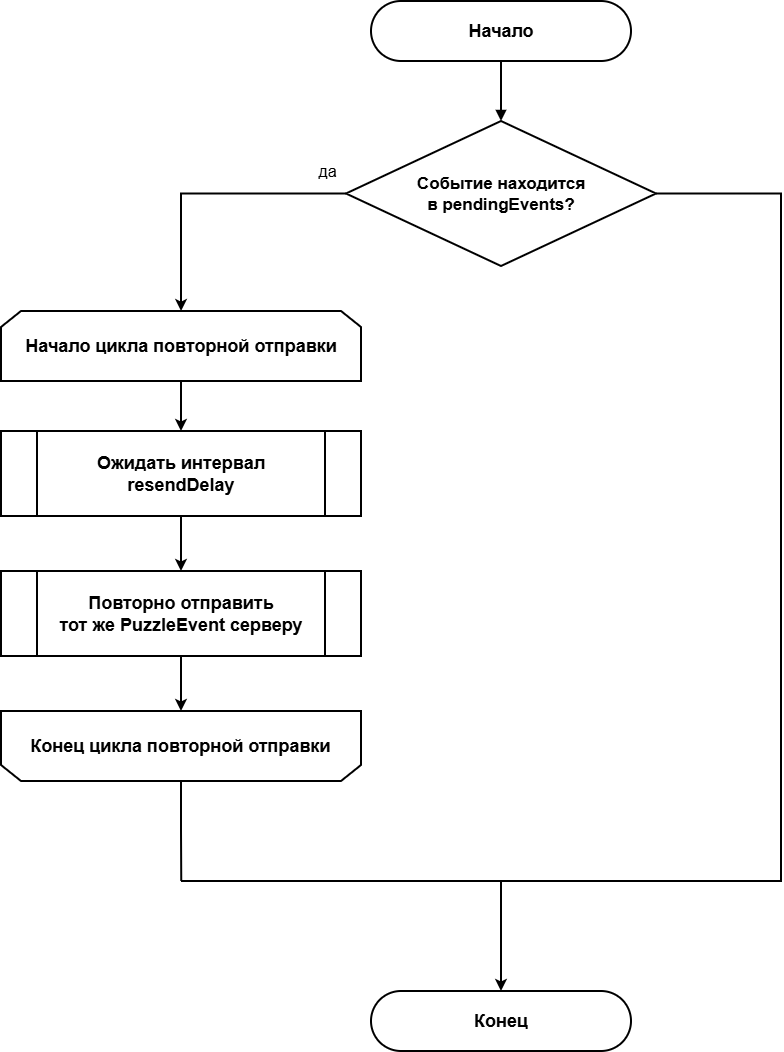
\includegraphics[height=0.72\textheight]{inc/img/recycle_event.png}
	\caption{Схема алгоритма повторной отправки неподтвержденных событий}
	\label{img:design-resend}
\end{figure}

\section{Структура программного обеспечения}

Для реализации предложенного метода разрабатываемое программное обеспечение должно включать следующие компоненты:
\begin{itemize}
	\item модуль сетевого обмена, выполняющий отправку и прием UDP-сообщений;
	\item модуль сериализации и десериализации сетевых сообщений;
	\item журнал неподтвержденных событий клиента;
	\item хранилище обработанных событий для фильтрации дубликатов;
	\item хранилище ожидаемых номеров последовательности на сервере;
	\item менеджер синхронизации событий;
	\item конечные автоматы игровых объектов;
	\item модель игрового состояния двух игроков.
\end{itemize}

Взаимодействие компонентов должно быть организовано так, чтобы сетевой модуль не изменял игровое состояние напрямую. Все входящие сообщения должны передаваться менеджеру синхронизации, который принимает решение о допустимости события и передает его целевому конечному автомату. Это разделяет транспортный уровень и уровень игровой логики, что снижает вероятность некорректного изменения состояния при ошибках сети.


\section*{Вывод}

В данном разделе был разработан метод обеспечения согласованности состояний двух асинхронных игроков с использованием событийной модели и конечных автоматов. 
Были сформулированы требования к методу, определена клиент-серверная функциональная модель синхронизации, задана формальная модель состояния игроков, игровых объектов, событий и сетевых сообщений.

Была предложена структура протокола синхронизации, включающая регистрацию клиента, формирование события, 
ожидание подтверждения, обработку события сервером, рассылку подтвержденного события, применение события клиентом, повторную отправку и отклонение некорректных событий. 
Для модели были описаны основные переходы и условия их выполнения.

\chapter{Технологический раздел}\label{implementation}

\section{Выбор средств программной реализации}

Для программной реализации метода была выбрана игровая среда Unity. Данный выбор обусловлен тем, что Unity предоставляет событийную модель выполнения сценариев, поддержку компонентов, механизм обработки пользовательского ввода, средства моделирования интерактивных сцен и возможность разработки логики на языке C\#~\cite{unity_monobehaviour}. Это позволяет реализовать не только сетевой обмен, но и программное обеспечение для проверки взаимодействия двух игроков.

В качестве языка программирования выбран C\#. Язык поддерживает объектно-ориентированную модель, обобщенные коллекции, перечисления, классы, интерфейсы и средства работы с сетевыми сокетами~\cite{csharp_reference}. Эти свойства используются при реализации конечных автоматов, событий, журналов неподтвержденных сообщений и сетевого транспортного уровня.

Для сетевого обмена выбран протокол UDP. Выбор UDP соответствует постановке задачи, так как метод должен работать в условиях отсутствия встроенных гарантий доставки и порядка сообщений. 
В реализации используется класс \texttt{UdpClient} пространства имен \texttt{System.Net.Sockets}, предоставляющий средства отправки и приема UDP-датаграмм~\cite{dotnet_udpclient}. 
Прикладная надежность реализуется через подтверждения, повторную отправку, контроль идентификаторов событий и проверку порядка сообщений.

\section{Структура программного обеспечения}

Разработанное программное обеспечение состоит из нескольких групп модулей:
\begin{itemize}
	\item модуль сетевого обмена;
	\item модуль синхронизации событий и конечных автоматов;
	\item модули объектов, реализующих интерфейс конечного автомата;
	\item модули пользовательского взаимодействия;
	\item модули сбора исследовательских метрик.
\end{itemize}

Основные классы программной реализации приведены в таблице~\ref{tab:implementation-modules}.

\begin{table}[H]
	\caption{Основные классы программной реализации}
	\label{tab:implementation-modules}
	\centering
	\small
	\renewcommand{\arraystretch}{1.2}
	\begin{tabular}{|p{6.2cm}|p{7.8cm}|}
		\hline
		Класс & Назначение \\ \hline
		\texttt{UdpEventTransport} & Отправка и прием UDP-сообщений, имитация потерь, задержки, вариативности задержки и дублирования пакетов \\ \hline
		\texttt{NetworkMessage} & Представление сетевого сообщения, содержащего игровое событие, подтверждение или служебное сообщение подключения \\ \hline
		\texttt{EventFsmSyncManager} & Центральный модуль синхронизации событий, обработки подтверждений, повторной отправки и применения событий к конечным автоматам \\ \hline
		\texttt{PuzzleEvent} & Представление логически значимого игрового события \\ \hline
		\texttt{IFsmPuzzleObject} & Интерфейс объектов, состояние которых изменяется через конечный автомат \\ \hline
		\texttt{PuzzleDoor} & Пример объекта, реализующего интерфейс \texttt{IFsmPuzzleObject} \\ \hline
		\texttt{ToggleBridge} & Пример объекта, реализующего интерфейс \texttt{IFsmPuzzleObject} \\ \hline
		\texttt{CoopHoldPuzzleController} & Пример объекта, реализующего интерфейс \texttt{IFsmPuzzleObject} для составного состояния взаимодействия \\ \hline
		\texttt{ColorSequenceController} & Пример объекта, реализующего интерфейс \texttt{IFsmPuzzleObject} для последовательной обработки событий \\ \hline
		\texttt{ResearchMetrics} & Сбор статистики отправки сообщений, потерь, повторных отправок, отклоненных дубликатов и примененных событий \\ \hline
	\end{tabular}
\end{table}


Структура программного обеспечения представлена в виде диаграммы классов на рисунке~\ref{img:implementation-class-diagram}. Конкретные классы игровых объектов на диаграмме рассматриваются не как самостоятельная предметная область, а как реализации общего интерфейса \texttt{IFsmPuzzleObject}, через который метод применяет подтвержденные события к конечным автоматам.

\begin{figure}[H]
	\centering
	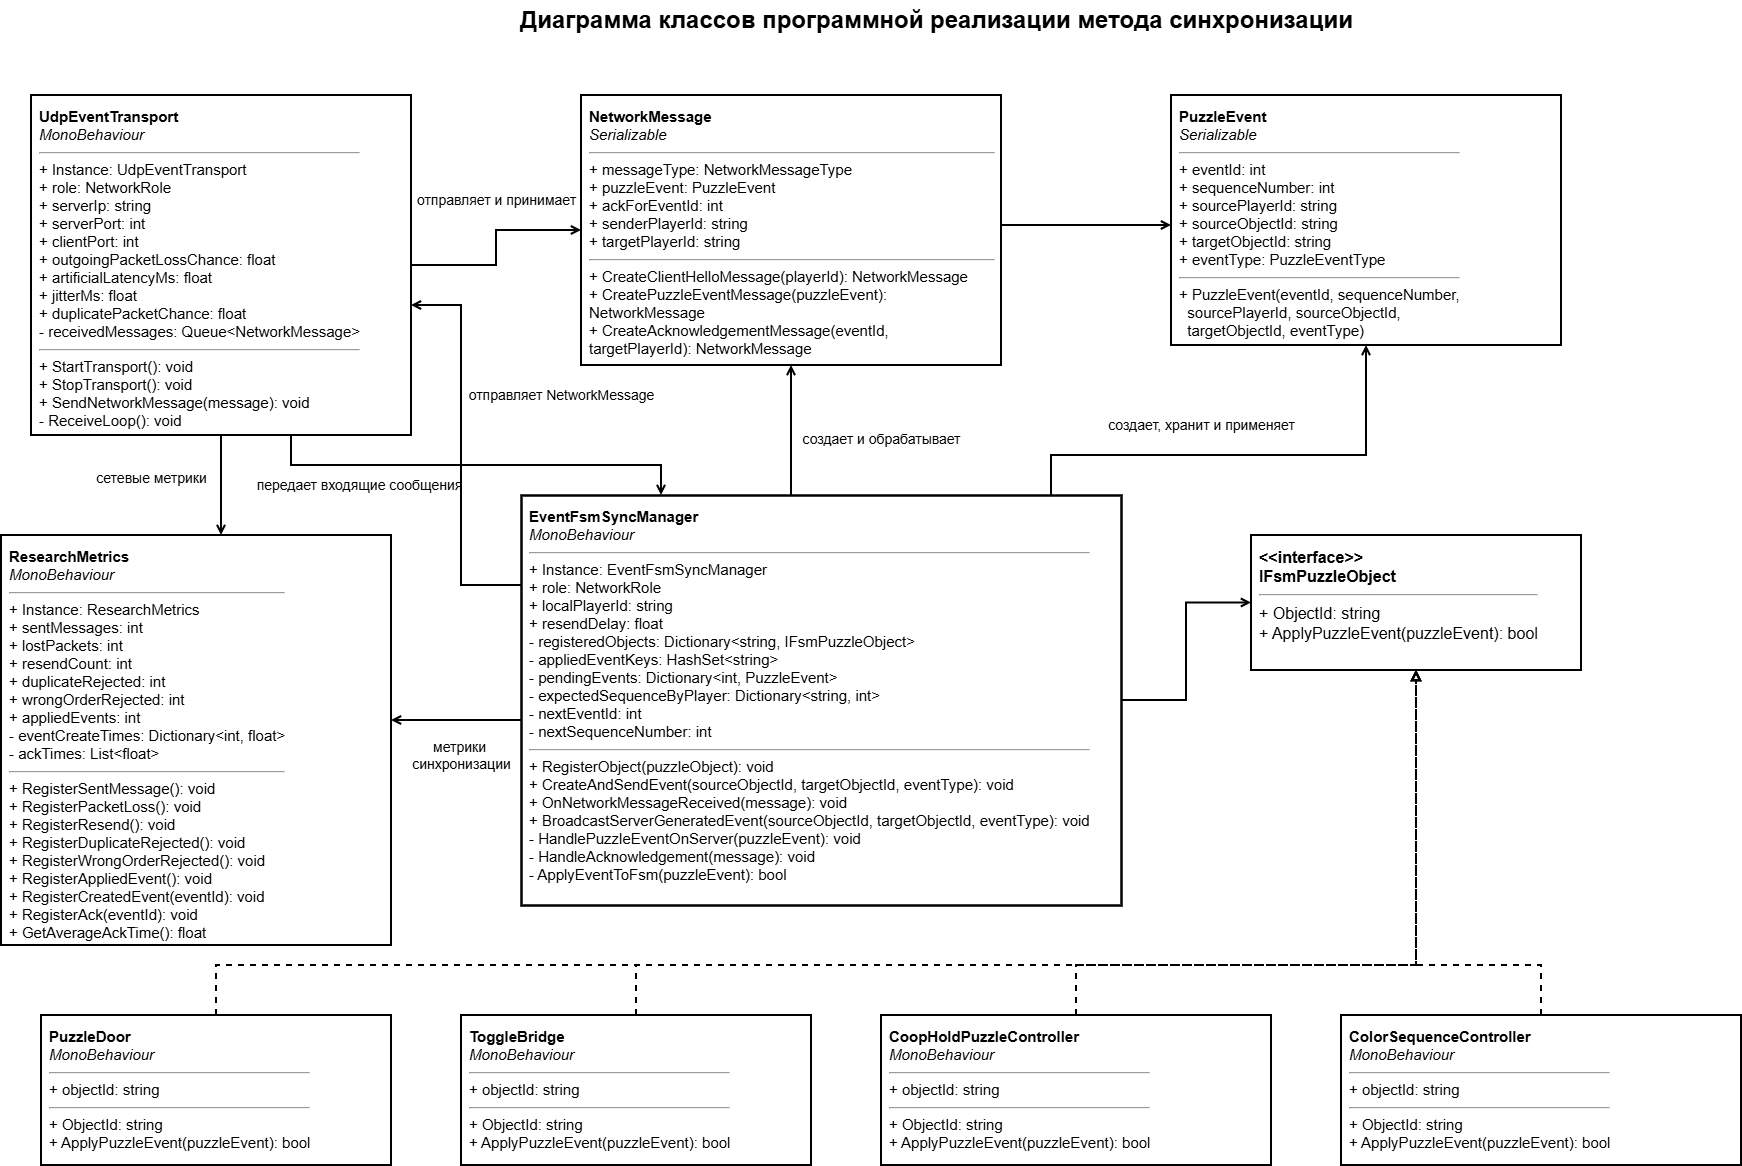
\includegraphics[width=\textwidth]{inc/img/class_diagram.png}
	\caption{Диаграмма классов программной реализации}
	\label{img:implementation-class-diagram}
\end{figure}

\section{Реализация сетевого обмена}

Сетевой обмен реализован в классе \texttt{UdpEventTransport}. Объект данного класса может работать в одной из двух ролей: \texttt{Server} или \texttt{Client}. 
Роль задается перечислением \texttt{NetworkRole}. Сервер открывает UDP-сокет на серверном порту и регистрирует адреса клиентов после получения служебного сообщения \texttt{ClientHello}. 
Клиент открывает собственный UDP-сокет, хранит адрес сервера и после запуска отправляет сообщение подключения.

При отправке сообщение типа \texttt{NetworkMessage} сериализуется в JSON-строку. Затем строка преобразуется в массив байтов и передается через UDP. Перед непосредственной отправкой применяется модель сетевых условий, включающая:
\begin{itemize}
	\item вероятность потери исходящего пакета;
	\item искусственную задержку отправки;
	\item вариативность задержки;
	\item вероятность дублирования пакета.
\end{itemize}

Прием UDP-сообщений выполняется в отдельном фоновом потоке. Это необходимо для того, чтобы ожидание входящих датаграмм не блокировало основной цикл Unity. 
Полученные сообщения помещаются в очередь \texttt{receivedMessages}. Доступ к очереди синхронизируется с помощью объекта блокировки. 
В методе \texttt{Update} сообщения извлекаются из очереди и передаются в \texttt{EventFsmSyncManager} уже в основном потоке Unity.

Игровые объекты, компоненты сцены и визуальное состояние должны изменяться из основного потока по правилам Unity. 
Поэтому фоновый поток отвечает только за сетевой прием, а изменение конечных автоматов и игровых объектов выполняется после передачи сообщения в основной цикл.

Фрагмент реализации отправки сообщения с учетом потерь, задержки, вариативности задержки и дублирования приведен в листинге~\ref{lst:udp-network-conditions}.

\sourcelisting[firstline=140,lastline=205]{../src/Networking/UdpEventTransport.cs}{Отправка UDP-сообщения с имитацией сетевых условий}{lst:udp-network-conditions}

Фрагмент приема сообщений в фоновом потоке и передачи их в основной поток Unity приведен в листинге~\ref{lst:udp-receive-loop}.

\sourcelisting[firstline=255,lastline=333]{../src/Networking/UdpEventTransport.cs}{Прием UDP-сообщений и обработка очереди в основном потоке}{lst:udp-receive-loop}

\section{Реализация структуры сетевого сообщения}

Сетевое сообщение представлено классом \texttt{NetworkMessage}. В реализации выделены три типа сообщений:
\begin{itemize}
	\item \texttt{ClientHello} --- служебное сообщение регистрации клиента;
	\item \texttt{PuzzleEvent} --- сообщение с игровым событием;
	\item \texttt{Acknowledgement} --- подтверждение обработки события.
\end{itemize}

Тип сообщения задается перечислением \texttt{NetworkMessageType}. Для создания сообщений используются статические методы:
\begin{itemize}
	\item \texttt{CreateClientHelloMessage};
	\item \texttt{CreatePuzzleEventMessage};
	\item \texttt{CreateAcknowledgementMessage}.
\end{itemize}

Игровое событие представлено классом \texttt{PuzzleEvent}. Событие содержит идентификатор, номер последовательности, идентификатор игрока-отправителя, идентификатор исходного объекта, 
идентификатор целевого объекта и тип события. Тип события задается перечислением \texttt{PuzzleEventType}.

Использование единого типа \texttt{PuzzleEvent} позволяет обрабатывать игровые события одинаковым образом независимо от того, к какому объекту сцены они относятся. Конкретная логика перехода состояния реализуется внутри целевого объекта, зарегистрированного в менеджере синхронизации.

Реализация структуры сетевого сообщения и фабричных методов создания сообщений приведена в листинге~\ref{lst:network-message}.

\sourcelisting{../src/Networking/NetworkMessage.cs}{Класс сетевого сообщения}{lst:network-message}

Структура игрового события приведена в листинге~\ref{lst:puzzle-event}.

\sourcelisting{../src/Method/PuzzleEvent.cs}{Класс игрового события}{lst:puzzle-event}

\section{Реализация менеджера синхронизации событий}

Основная логика метода реализована в классе \texttt{EventFsmSyncManager}. Данный класс выполняет следующие функции:
\begin{itemize}
	\item регистрацию объектов, реализующих интерфейс \texttt{IFsmPuzzleObject};
	\item создание локальных игровых событий;
	\item присвоение событию идентификатора и номера последовательности;
	\item отправку события через транспортный уровень;
	\item хранение неподтвержденных событий;
	\item повторную отправку события при отсутствии подтверждения;
	\item обработку входящих событий на сервере;
	\item обработку подтвержденных сервером событий на клиенте;
	\item фильтрацию дубликатов;
	\item контроль порядка событий от каждого игрока;
	\item применение события к целевому конечному автомату.
\end{itemize}

Для хранения объектов, состояние которых изменяется через конечные автоматы, используется словарь \texttt{registeredObjects}. 
Ключом является строковый идентификатор объекта, значением --- объект, реализующий интерфейс \texttt{IFsmPuzzleObject}. 
Благодаря этому сетевое событие может быть доставлено конкретному объекту по полю \texttt{targetObjectId}.

Для защиты от повторной обработки используется множество \texttt{appliedEventKeys}. Ключ события формируется из идентификатора игрока-отправителя и идентификатора события. 
Если событие с таким ключом уже было применено, повторный пакет не изменяет состояние конечного автомата.

Для реализации подтверждений используется словарь \texttt{pendingEvents}. В нем хранятся события, отправленные клиентом, но еще не подтвержденные сервером. 
После получения сообщения \texttt{Acknowledgement} соответствующее событие удаляется из словаря.

Для контроля порядка сообщений используется словарь \texttt{expectedSequenceByPlayer}. Для каждого игрока хранится номер следующего ожидаемого события. 
Если сервер получает событие с меньшим номером, оно считается устаревшим. Если получен номер больше ожидаемого, событие считается пришедшим раньше недостающих событий и не применяется.

Фрагмент создания события, присвоения идентификатора, сохранения в журнале неподтвержденных событий и запуска повторной отправки приведен в листинге~\ref{lst:create-send-event}.

\sourcelisting[firstline=91,lastline=148]{../src/Method/EventFsmSyncManager.cs}{Создание события и повторная отправка до подтверждения}{lst:create-send-event}

Фрагмент обработки события на сервере приведен в листинге~\ref{lst:server-event-handling}.

\sourcelisting[firstline=258,lastline=336]{../src/Method/EventFsmSyncManager.cs}{Проверка порядка и подтверждение события на сервере}{lst:server-event-handling}

\section{Реализация подтверждений и повторной отправки}

После создания события клиент сохраняет его в \texttt{pendingEvents}, отправляет сообщение \texttt{PuzzleEvent} и запускает корутину \texttt{ResendUntilAcknowledged}. 
Пока событие присутствует в словаре неподтвержденных событий, корутина ожидает интервал \texttt{resendDelay} и повторно отправляет то же самое событие.

Повторно отправляемое событие сохраняет исходные значения \texttt{eventId} и \texttt{sequenceNumber}. 
Это необходимо, потому что повторная отправка не должна восприниматься системой как новое игровое действие. Если получатель уже применил событие, он распознает дубликат и не изменяет состояние повторно.

Сервер после успешной проверки и применения события отправляет клиенту подтверждение. Подтверждение содержит идентификатор события и идентификатор игрока, которому оно адресовано. Клиент принимает подтверждение только в том случае, если поле \texttt{targetPlayerId} совпадает с его локальным идентификатором.

Фрагмент обработки подтверждения на стороне клиента приведен в листинге~\ref{lst:ack-handling}.

\sourcelisting[firstline=210,lastline=256]{../src/Method/EventFsmSyncManager.cs}{Обработка подтверждения и удаление события из журнала ожидания}{lst:ack-handling}

\section{Реализация объектов с конечными автоматами}

Каждый игровой объект, состояние которого изменяется через сетевое событие, реализует интерфейс \texttt{IFsmPuzzleObject}. Интерфейс содержит свойство \texttt{ObjectId} и метод \texttt{ApplyPuzzleEvent}. Такой подход позволяет отделить общий механизм сетевой синхронизации от конкретной игровой логики.

При запуске объект регистрируется в \texttt{EventFsmSyncManager} вызовом метода \texttt{RegisterObject}. Менеджер сохраняет объект в словаре \texttt{registeredObjects}, где ключом является строковый идентификатор \texttt{ObjectId}. После получения подтвержденного события менеджер находит целевой объект по полю \texttt{targetObjectId} и вызывает метод \texttt{ApplyPuzzleEvent}.

В разработанном программном обеспечении классы \texttt{PuzzleDoor}, \texttt{ToggleBridge}, \texttt{CoopHoldPuzzleController} и \texttt{ColorSequenceController} выступают как примеры объектов, 
подключаемых к методу через единый интерфейс. Их внутренняя логика может различаться, однако для алгоритма синхронизации все такие объекты не отличаются,
они предоставляют идентификатор и возвращают результат применения события. Это позволяет рассматривать конкретные игровые сценарии как заменяемые реализации целевого конечного автомата, 
не изменяющие транспортный уровень и механизм согласования состояний.

Интерфейс синхронизируемого объекта приведен в листинге~\ref{lst:fsm-interface}.

\sourcelisting{../src/Method/IFsmPuzzleObject.cs}{Интерфейс объекта с конечным автоматом}{lst:fsm-interface}

Пример реализации объекта с конечным автоматом приведен в листинге~\ref{lst:puzzle-door}.

\sourcelisting[firstline=4,lastline=65]{../src/Interactables/PuzzleDoor.cs}{Регистрация и обработка события объектом \texttt{PuzzleDoor}}{lst:puzzle-door}

\section{Реализация пользовательского взаимодействия}

Пользовательское взаимодействие реализовано через интерактивные объекты сцены. Объекты, с которыми может взаимодействовать игрок, преобразуют локальное действие в вызов \texttt{CreateAndSendEvent}.
При этом локальное действие не передается по сети напрямую, оно сначала приводится к типизированному событию \texttt{PuzzleEvent}, содержащему идентификаторы источника, цели, игрока и тип операции.

Таким образом, пользовательское действие не изменяет состояние удаленного объекта напрямую. Оно преобразуется в событие, которое проходит через общий механизм сетевой синхронизации и только после проверки применяется к целевому конечному автомату.

\section{Средства имитации сетевых ошибок}

Для проверки устойчивости метода в транспортном модуле реализованы параметры искусственного ухудшения сети:
\begin{itemize}
	\item \texttt{outgoingPacketLossChance} --- вероятность потери исходящего пакета;
	\item \texttt{artificialLatencyMs} --- средняя искусственная задержка отправки;
	\item \texttt{jitterMs} --- разброс задержки;
	\item \texttt{duplicatePacketChance} --- вероятность отправки дубликата.
\end{itemize}

Эти параметры задаются в инспекторе Unity и позволяют моделировать нестабильное сетевое соединение без изменения основного алгоритма. При имитации потери сообщение не отправляется в сеть. При имитации задержки отправка откладывается на заданное время. При имитации дубликата тот же массив байтов отправляется повторно через небольшой интервал.

Сбор статистики выполняется классом \texttt{ResearchMetrics}. Он регистрирует количество отправленных сообщений, имитированных потерь, повторных отправок, отклоненных дубликатов, событий с нарушением порядка и успешно примененных событий. Также сохраняется время создания события и время получения подтверждения, что позволяет вычислять среднее время подтверждения.

Фрагмент регистрации метрик и вычисления среднего времени подтверждения приведен в листинге~\ref{lst:research-metrics}.

\sourcelisting[firstline=34,lastline=99]{../src/Research/ResearchMetrics.cs}{Сбор исследовательских метрик}{lst:research-metrics}

\section{Тестирование разработанного программного обеспечения}

Тестирование разработанного программного обеспечения выполнялось с использованием ручных сценариев, проверяющих основные функции метода синхронизации и корректность обработки сетевых ошибок. Для каждого сценария проверялось состояние целевого конечного автомата и сообщения журнала выполнения Unity.

Основные тестовые сценарии приведены в таблице~\ref{tab:implementation-tests}.

\begin{table}[H]
	\caption{Сценарии тестирования программной реализации}
	\label{tab:implementation-tests}
	\centering
	\renewcommand{\arraystretch}{1.2}
	\begin{tabular}{|p{4cm}|p{5cm}|p{5cm}|}
		\hline
		Сценарий & Действие & Ожидаемый результат \\ \hline
		Доставка события & Игрок взаимодействует с интерактивным объектом & Создается событие, сервер применяет его к конечному автомату, клиент получает подтверждение \\ \hline
		Повторная отправка & Для исходящих пакетов задается вероятность потери & При отсутствии подтверждения событие повторно отправляется с тем же идентификатором \\ \hline
		Фильтрация дубликата & Включается вероятность дублирования пакета & Дубликат события не изменяет состояние повторно \\ \hline
		Контроль порядка & Отправляется событие с номером больше ожидаемого & Событие не применяется до восстановления порядка \\ \hline
		Недопустимое событие & Событие направляется объекту, для которого его тип не подходит & Метод \texttt{ApplyPuzzleEvent} возвращает отрицательный результат, состояние объекта не изменяется \\ \hline
		Синхронизация FSM-объекта & Оба игрока формируют события для одного синхронизируемого объекта & На обеих сторонах фиксируется одинаковое логическое состояние объекта \\ \hline
	\end{tabular}
\end{table}

Сценарии тестирования проверяют не отдельные игровые действия, а свойства метода: доставку критичного события, повторную отправку, фильтрацию дубликатов, контроль порядка и сохранение согласованного состояния конечного автомата.

\section*{Вывод}

В данном разделе был обоснован выбор Unity, языка C\# и UDP-сетевого обмена для программной реализации метода обеспечения согласованности состояний двух асинхронных игроков. Была описана структура программного обеспечения, включающая транспортный уровень, менеджер синхронизации событий, представление сетевых сообщений, интерфейс объектов с конечными автоматами и средства сбора статистики.

Были рассмотрены детали реализации прикладной надежности поверх UDP, такие как подтверждение обработки события, хранение неподтвержденных событий, повторная отправка, фильтрация дубликатов и контроль порядка сообщений. 
Также был описан способ подключения объектов, реализующих интерфейс \texttt{IFsmPuzzleObject}, и сценарии тестирования разработанного программного обеспечения.

\chapter{Исследовательский раздел}\label{research}

\section{Цель исследования}

Целью исследования является оценка эффективности разработанного метода синхронизации состояний двух игроков и его сравнение с базовой событийной синхронизацией без прикладной надежности.

В рамках исследования необходимо:
\begin{itemize}
	\item определить критерии оценки эффективности синхронизации состояний;
	\item задать параметры сетевой среды для экспериментальных запусков;
	\item выполнить серию испытаний для разработанного метода и базового UDP-подхода;
	\item оценить долю успешно примененных событий;
	\item оценить среднее время подтверждения или возврата события;
	\item оценить количество повторных отправок, возникающих при потере сообщений;
	\item определить влияние дублирования пакетов на повторную обработку событий;
	\item сравнить устойчивость двух подходов к потере, задержке и дублированию UDP-пакетов.
\end{itemize}

\section{Сравниваемые режимы синхронизации}

Для проведения исследования в разработанном программном обеспечении реализованы два режима синхронизации, выбираемые параметром \texttt{SynchronizationResearchMode}. Режим \texttt{ReliableFsmMethod} соответствует разработанному методу. Режим \texttt{BasicUdpEvents} используется как контрольный вариант и моделирует простую событийную передачу по UDP без подтверждений и повторной отправки.

Сравнение выполняется при одинаковых входных событиях и одинаковых параметрах сетевой среды. Это позволяет исключить влияние различий в игровой логике и сравнивать именно сетевые и алгоритмические механизмы синхронизации.

\begin{table}[H]
	\caption{Сравниваемые режимы синхронизации}
	\label{tab:research-modes}
	\centering
	\small
	\renewcommand{\arraystretch}{1.2}
	\begin{tabular}{|p{3.4cm}|p{4.6cm}|p{4.6cm}|}
		\hline
		Механизм & Базовая событийная UDP-синхронизация & Разработанный метод \\ \hline
		Режим синхронизации & \texttt{BasicUdpEvents} & \texttt{ReliableFsmMethod} \\ \hline
		Передача события & Однократная отправка события & Отправка события с регистрацией ожидания подтверждения \\ \hline
		Подтверждение обработки & Не используется & Используется сообщение \texttt{Acknowledgement} \\ \hline
		Повторная отправка & Не выполняется & Выполняется после истечения \texttt{resendDelay} \\ \hline
		Фильтрация дубликатов & Не выполняется на уровне метода & Выполняется по ключу события \\ \hline
		Контроль порядка & Не выполняется & Выполняется по \texttt{sequenceNumber} \\ \hline
		Защита состояния FSM & Не выполняется & Обеспечивается проверкой порядка, подтверждением и повторной отправкой \\ \hline
	\end{tabular}
\end{table}

В базовом режиме событие, потерянное на транспортном уровне, не восстанавливается. Если сообщение было продублировано, оно может быть повторно передано в обработчик конечного автомата. В разработанном методе потеря события или подтверждения приводит к повторной отправке, а повторное получение уже обработанного события не изменяет состояние конечного автомата.

\section{Критерии оценки эффективности}

Для оценки используются метрики, собираемые при выполнении разработанного программного обеспечения классом \texttt{ResearchMetrics}. Метрики фиксируются отдельно для каждого запуска и выводятся в журнал приложения после завершения автоматического теста.

К основным метрикам относятся:
\begin{itemize}
	\item $N_{created}$ --- количество созданных логически значимых событий;
	\item $N_{sent}$ --- количество фактически отправленных сетевых сообщений;
	\item $N_{lost}$ --- количество имитированных потерь исходящих UDP-пакетов;
	\item $N_{resend}$ --- количество повторных отправок событий;
	\item $N_{dup}$ --- количество отклоненных дубликатов;
	\item $N_{wrong}$ --- количество событий, отклоненных из-за нарушения порядка;
	\item $N_{applied}$ --- количество событий, примененных к конечному автомату;
	\item $T_{ack}^{avg}$ --- среднее время подтверждения или возврата события.
\end{itemize}

Для разработанного метода величина $T_{ack}^{avg}$ соответствует среднему времени получения подтверждения \texttt{Acknowledgement}. Для базового режима эта величина интерпретируется как среднее время возврата события от серверной стороны к клиенту, поскольку отдельное сообщение подтверждения в данном режиме не используется.

Среднее время подтверждения или возврата события определяется выражением:
\[
	T_{ack}^{avg} = \frac{1}{N}\sum_{i=1}^{N}(t_i^{ack} - t_i^{send}),
\]
где:
\begin{itemize}
	\item $N$ --- количество событий, для которых был получен ответ;
	\item $t_i^{send}$ --- момент создания события;
	\item $t_i^{ack}$ --- момент получения подтверждения или подтвержденного сервером события.
\end{itemize}

Доля примененных событий определяется как:
\[
	K_{applied} = \frac{N_{applied}}{N_{created}}.
\]

Для разработанного метода ожидаемым значением $K_{applied}$ является значение, близкое к единице. Для базового режима при потере пакетов значение $K_{applied}$ может уменьшаться, так как потерянные события не восстанавливаются. При дублировании пакетов в базовом режиме показатель может превышать единицу, что указывает на повторную обработку одного и того же события.

Относительное количество повторных отправок определяется как:
\[
	K_{resend} = \frac{N_{resend}}{N_{created}}.
\]

Рост $K_{resend}$ при наличии потерь является ожидаемым для разработанного метода, так как дополнительные сообщения используются для восстановления доставки критичных событий. 
Для базового UDP-подхода $K_{resend}$ равно нулю, однако отсутствие повторов в этом случае не является преимуществом, так как потерянные события не компенсируются.

\section{Порядок проведения исследования}

Автоматизация испытаний выполняется компонентом \texttt{AutomatedResearchTest}. Компонент создает 100 событий с интервалом 0.2~с. После завершения генерации событий выполняется ожидание завершения сетевой обработки, затем компонент \texttt{ResearchMetrics} выводит итоговые значения метрик.

Параметры сетевой среды задаются в компоненте \texttt{UdpEventTransport}:
\begin{itemize}
	\item \texttt{outgoingPacketLossChance} --- вероятность потери исходящего пакета;
	\item \texttt{artificialLatencyMs} --- искусственная задержка отправки;
	\item \texttt{jitterMs} --- вариативность задержки;
	\item \texttt{duplicatePacketChance} --- вероятность дублирования отправляемого пакета.
\end{itemize}

Для каждого сценария выполняются два запуска: один в режиме \texttt{ReliableFsmMethod}, второй в режиме \texttt{BasicUdpEvents}. Значения параметров сетевой среды в двух запусках совпадают.

\section{Сценарии исследования}

Для исследования выбраны сценарии, отражающие типовые условия сетевого взаимодействия в многопользовательском приложении. Сценарии приведены в таблице~\ref{tab:research-scenarios}.

\begin{table}[H]
	\caption{Сценарии исследования UDP-обмена}
	\label{tab:research-scenarios}
	\centering
	\renewcommand{\arraystretch}{1.2}
	\begin{tabular}{|p{4cm}|c|c|c|c|}
		\hline
		Сценарий & Потери, \% & Задержка, мс & Jitter, мс & Дубликаты, \% \\ \hline
		Стабильная сеть & 0 & 0 & 0 & 0 \\ \hline
		Умеренная задержка & 0 & 100 & 20 & 0 \\ \hline
		Потери пакетов & 5 & 100 & 20 & 0 \\ \hline
		Высокие потери & 15 & 100 & 30 & 0 \\ \hline
		Дублирование пакетов & 0 & 100 & 20 & 20 \\ \hline
		Нестабильная сеть & 10 & 150 & 50 & 10 \\ \hline
	\end{tabular}
\end{table}

Первые два сценария используются для оценки влияния задержки без потери сообщений. Сценарии с потерями позволяют оценить способность метода восстанавливать доставку критичных событий. Сценарий с дублированием проверяет устойчивость к повторному получению одного и того же события. Нестабильная сеть объединяет задержку, вариативность задержки, потерю и дублирование пакетов.

\section{Результаты исследования разработанного метода}

В таблице~\ref{tab:research-reliable-results} приведены результаты запусков для режима \texttt{ReliableFsmMethod}. 

\begin{table}[H]
	\caption{Результаты исследования разработанного метода}
	\label{tab:research-reliable-results}
	\centering
	\small
	\renewcommand{\arraystretch}{1.2}
	\begin{tabular}{|p{3.2cm}|c|c|c|c|c|c|}
		\hline
		Сценарий & Создано & Отправлено & Потери & Повторы & Применено & $T_{ack}^{avg}$, с \\ \hline
		Стабильная сеть & 100 & 102 & 0 & 2 & 100 & 0.099 \\ \hline
		Умеренная задержка & 100 & 118 & 0 & 18 & 100 & 0.332 \\ \hline
		Потери пакетов & 100 & 146 & 8 & 54 & 100 & 0.939 \\ \hline
		Высокие потери & 100 & 132 & 20 & 46 & 99 & 0.711 \\ \hline
		Дублирование пакетов & 100 & 131 & 0 & 12 & 100 & 0.362 \\ \hline
		Нестабильная сеть & 100 & 139 & 8 & 38 & 99 & 0.548 \\ \hline
	\end{tabular}
\end{table}

Из таблицы видно, что при стабильной сети метод обеспечивает применение всех созданных событий. При увеличении задержки возрастает среднее время подтверждения, 
однако доля примененных событий остается равной единице. При появлении потерь возрастает количество повторных отправок, что является следствием работы механизма восстановления доставки. 
В сценариях с высокими потерями и нестабильной сетью часть событий может не попасть в окно наблюдения, однако механизм повторной отправки продолжает работу до получения подтверждения.

Важным результатом является то, что увеличение числа отправленных сообщений не приводит к повторному изменению состояния конечного автомата. 
Повторные отправки и дубликаты распознаются по ключу события и используются только для восстановления факта доставки и подтверждения обработки.

\section{Результаты исследования базового UDP-подхода}

В таблице~\ref{tab:research-basic-results} приведены результаты запусков для режима \texttt{BasicUdpEvents}. В этом режиме событие отправляется один раз, не помещается в журнал неподтвержденных событий и не отправляется повторно.

\begin{table}[H]
	\caption{Результаты исследования базовой событийной UDP-синхронизации}
	\label{tab:research-basic-results}
	\centering
	\small
	\renewcommand{\arraystretch}{1.2}
	\begin{tabular}{|p{3.2cm}|c|c|c|c|c|c|}
		\hline
		Сценарий & Создано & Отправлено & Потери & Повторы & Применено & $T_{ack}^{avg}$, с \\ \hline
		Стабильная сеть & 100 & 100 & 0 & 0 & 100 & 0.086 \\ \hline
		Умеренная задержка & 100 & 100 & 0 & 0 & 100 & 0.301 \\ \hline
		Потери пакетов & 100 & 95 & 5 & 0 & 91 & 0.314 \\ \hline
		Высокие потери & 100 & 85 & 15 & 0 & 73 & 0.327 \\ \hline
		Дублирование пакетов & 100 & 120 & 0 & 0 & 124 & 0.309 \\ \hline
		Нестабильная сеть & 100 & 101 & 10 & 0 & 88 & 0.423 \\ \hline
	\end{tabular}
\end{table}

При отсутствии потерь базовый подход способен доставить все события, так как сетевой канал не создает отказов. Однако при потере пакетов доля примененных событий снижается, поскольку потерянное событие не восстанавливается. При дублировании пакетов количество применений может превышать число созданных событий, что свидетельствует о повторной обработке одного и того же логического действия.

\section{Сравнение результатов}

Сводное сравнение двух режимов приведено в таблице~\ref{tab:research-comparison}. 
Для сравнения используется доля примененных событий $K_{applied}$. Для разработанного метода значение, близкое к единице, означает доставку и обработку созданных событий. 
Для базового подхода значение меньше единицы означает потерю событий, а значение больше единицы --- повторную обработку из-за дублирования.

\begin{table}[H]
	\caption{Сравнение разработанного метода с базовой UDP-синхронизацией}
	\label{tab:research-comparison}
	\centering
	\small
	\renewcommand{\arraystretch}{1.2}
	\begin{tabular}{|p{5cm}|c|c|}
		\hline
		Сценарий & $K_{applied}$ базового подхода & $K_{applied}$ разработанного метода \\ \hline
		Стабильная сеть & 1.00 & 1.00 \\ \hline
		Умеренная задержка & 1.00 & 1.00 \\ \hline
		Потери пакетов & 0.91 & 1.00 \\ \hline
		Высокие потери & 0.73 & 0.99 \\ \hline
		Дублирование пакетов & 1.24 & 1.00 \\ \hline
		Нестабильная сеть & 0.88 & 0.99 \\ \hline
	\end{tabular}
\end{table}

Результаты показывают, что при благоприятных сетевых условиях оба подхода дают сопоставимый результат. Это ожидаемо, поскольку при отсутствии потерь 
и дубликатов простая передача события достаточна для сохранения состояния. Отличие проявляется при появлении сетевых ошибок.

При потере пакетов базовый подход теряет часть событий без возможности восстановления. 
Разработанный метод компенсирует такие потери повторной отправкой. При дублировании пакетов базовый подход допускает повторную обработку события, 
тогда как разработанный метод распознает уже обработанное событие и не изменяет конечный автомат повторно.

\section{Выводы по результатам исследования}

По результатам исследования можно сделать следующие выводы:
\begin{itemize}
	\item при стабильной сети разработанный метод и базовая событийная UDP-синхронизация обеспечивают применение всех событий;
	\item при увеличении задержки возрастает среднее время подтверждения, однако согласованность состояний сохраняется;
	\item при потере пакетов базовый подход теряет часть событий, так как не содержит механизма восстановления доставки;
	\item разработанный метод компенсирует потерю сообщений за счет хранения событий в \texttt{pendingEvents} и повторной отправки после истечения времени ожидания;
	\item при дублировании пакетов базовый подход может привести к повторной обработке одного и того же события;
	\item фильтрация дубликатов и контроль порядка в разработанном методе предотвращают повторное и несогласованное изменение конечного автомата;
	\item увеличение числа отправленных сообщений в разработанном методе является ожидаемым следствием обеспечения прикладной надежности поверх UDP.
\end{itemize}

\section*{Вывод}

В данном разделе были определены критерии оценки эффективности разработанного метода, описаны режимы экспериментального сравнения и заданы сценарии исследования UDP-сетевого обмена. Было проведено сравнение разработанного метода с базовой событийной UDP-синхронизацией без прикладной надежности.

Результаты исследования показывают, что базовый подход достаточен только при отсутствии сетевых ошибок. При потере и дублировании пакетов он не гарантирует ни доставку критичного события, ни его однократную обработку. Разработанный метод вводит дополнительные служебные механизмы: подтверждения, повторную отправку, контроль порядка и фильтрацию дубликатов. Эти механизмы увеличивают количество сетевых сообщений, однако позволяют сохранять согласованность состояний конечного автомата в условиях ненадежного UDP-обмена.

\chapter*{ЗАКЛЮЧЕНИЕ}
\addcontentsline{toc}{chapter}{ЗАКЛЮЧЕНИЕ}

В результате выполнения выпускной квалификационной работы был разработан метод обеспечения согласованности состояний двух асинхронных игроков с помощью конечных автоматов.

В ходе выполнения работы были решены следующие задачи:
\begin{itemize}
	\item проведен анализ предметной области синхронизации игровых состояний и передачи данных в многопользовательских играх;
	\item рассмотрены существующие подходы к синхронизации состояний и способы передачи игровых данных;
	\item описаны типовые игровые данные, подлежащие хранению и передаче;
	\item определены основные причины рассинхронизации игровых состояний;
	\item разработан метод синхронизации состояний двух игроков с использованием конечных автоматов;
	\item определена формальная модель состояний системы, событий и переходов между состояниями;
	\item разработана структура конечного автомата, описывающего взаимодействие игроков;
	\item представлен алгоритм синхронизации состояний, включающий обработку входящих и исходящих событий, подтверждения доставки и повторную отправку сообщений;
	\item обоснован выбор Unity, языка C\# и UDP-сетевого обмена в качестве средств программной реализации;
	\item разработано программное обеспечение, реализующее предложенный метод синхронизации;
	\item разработано программное обеспечение для взаимодействия игроков на основе событий и конечных автоматов;
	\item проведено тестирование разработанного программного обеспечения;
	\item определены критерии оценки эффективности разработанного метода;
	\item разработана методика исследования эффективности метода при различных параметрах сетевого взаимодействия;
	\item выполнено сравнение разработанного метода с событийной синхронизацией без механизмов прикладной надежности.
\end{itemize}

Разработанный метод рассматривает синхронизацию не как простую передачу состояния между клиентом и сервером, 
а как задачу согласованного выполнения событий в распределенной асинхронной системе. Для этого логика взаимодействия игроков представлена в виде конечного автомата, 
а каждое значимое игровое действие обрабатывается как событие, допустимость которого проверяется относительно текущего состояния системы.

В программной реализации поверх UDP-сетевого обмена были реализованы механизмы прикладной надежности, такие как подтверждение обработки событий, 
хранение неподтвержденных событий, повторная отправка при отсутствии подтверждения, фильтрация дубликатов и контроль порядка сообщений. 
Эти механизмы позволяют снизить влияние потерь, дублирования и нарушения порядка доставки пакетов на корректность логического состояния игроков.


\makebibliography

\chapter*{\begin{center}
		\vspace{-2.5em}	ПРИЛОЖЕНИЕ А\vspace{-2em}
	\end{center}
}
\addcontentsline{toc}{chapter}{\MakeUppercase{ПРИЛОЖЕНИЕ А}}


\end{document}
